%%%%%%%%%%%%%%%%%%%% book.tex %%%%%%%%%%%%%%%%%%%%%%%%%%%%%
%
% sample root file for the chapters of your "monograph"
%
% Use this file as a template for your own input.
%
%%%%%%%%%%%%%%%% Springer-Verlag %%%%%%%%%%%%%%%%%%%%%%%%%%


% RECOMMENDED %%%%%%%%%%%%%%%%%%%%%%%%%%%%%%%%%%%%%%%%%%%%%%%%%%%
\documentclass[envcountsame,envcountchap, openany]{mysvmono}
\usepackage[margin=1in]{geometry}
\usepackage[T5]{fontenc}

\usepackage[utf8]{inputenc}
\usepackage{amsmath}
\usepackage{amssymb}
\setlength{\parindent}{0em}
\setlength{\parskip}{1em}
% choose options for [] as required from the list
% in the Reference Guide, Sect. 2.2

\usepackage{makeidx}         % allows index generation
\usepackage{graphicx}        % standard LaTeX graphics tool
                             % when including figure files
\usepackage{multicol}        % used for the two-column index
\usepackage[bottom]{footmisc}% places footnotes at page bottom
% etc.
% see the list of further useful packages
% in the Reference Guide, Sects. 2.3, 3.1-3.3

\makeindex             % used for the subject index
                       % please use the style svind.ist with
                       % your makeindex program

\usepackage{cite,url,bm,hyperref}
\usepackage{hyperref}
\hypersetup{
    colorlinks=true,
    linkcolor=blue,
    filecolor=magenta,      
    urlcolor=blue,
}

%%%%%%%%%%%%%%%%%%%5
\usepackage{listings}
\usepackage{color}

%New colors defined below
\definecolor{codegreen}{rgb}{0,0.6,0}
\definecolor{codegray}{rgb}{0.5,0.5,0.5}
\definecolor{codepurple}{rgb}{0.58,0,0.82}
\definecolor{backcolour}{rgb}{0.95,0.95,0.92}


\usepackage{courier}

\lstset{columns=flexible}

%Code listing style named "mystyle"
\lstdefinestyle{mystyle}{
  backgroundcolor=\color{backcolour},   commentstyle=\color{codegreen},
  keywordstyle=\color{magenta},
  stringstyle=\color{codepurple},
  basicstyle=\footnotesize,
  breakatwhitespace=false,         
  breaklines=true,                 
  captionpos=b,                    
  keepspaces=true,                 
  showspaces=true,                
  showstringspaces=false,
  showtabs=false,                  
  tabsize=2, 
  basicstyle=\footnotesize\ttfamily,
}
\makeatletter
\def\lst@outputspace{{\ifx\lst@bkgcolor\empty\color{white}\else\lst@bkgcolor\fi\lst@visiblespace}}
\makeatother

\lstset{basicstyle=\footnotesize\ttfamily,breaklines=true}

%"mystyle" code listing set
\lstset{style=mystyle}
%%%%%%%%%%%%%%%%%%%
\usepackage[font={normalsize}]{caption}
%%%%%%%%%%%%%%%%%%%%%%%%%%%%%%%%%%%%%%%%%%%%%%%%%%%%%%%%%%%%%%%%%%%%%

% Default fixed font does not support bold face
\DeclareFixedFont{\ttb}{T1}{txtt}{bx}{n}{10} % for bold
\DeclareFixedFont{\ttm}{T1}{txtt}{m}{n}{10}  % for normal

% Custom colors
\usepackage{color}
\definecolor{deepblue}{rgb}{0,0,0.5}
\definecolor{deepred}{rgb}{0.6,0,0}
\definecolor{deepgreen}{rgb}{0,0.5,0}

\usepackage{listings}

% Python style for highlighting
\newcommand\pythonstyle{\lstset{
language=Python,
basicstyle=\ttm,
otherkeywords={self},             % Add keywords here
keywordstyle=\ttb\color{deepblue},
emph={MyClass,__init__},          % Custom highlighting
emphstyle=\ttb\color{deepred},    % Custom highlighting style
stringstyle=\color{deepgreen},
frame=tb,                         % Any extra options here
showstringspaces=false            % 
}}


% Python environment
\lstnewenvironment{python}[1][]
{
\pythonstyle
\lstset{#1}
}
{}

% Python for external files
\newcommand\pythonexternal[2][]{{
\pythonstyle
\lstinputlisting[#1]{#2}}}

% Python for inline
\newcommand\pythoninline[1]{{\pythonstyle\lstinline!#1!}}



\begin{document}

\author{Vũ Hữu Tiệp}
\title{\bf Machine Learning cơ bản\\
{\small First Edition}}
% }
% \subtitle{-- Monograph --}
\maketitle

\frontmatter%%%%%%%%%%%%%%%%%%%%%%%%%%%%%%%%%%%%%%%%%%%%%%%%%%%%%%

% 
%%%%%%%%%%%%%%%%%%%%%%% dedic.tex %%%%%%%%%%%%%%%%%%%%%%%%%%%%%%%%%
%
% sample dedication
%
% Use this file as a template for your own input.
%
%%%%%%%%%%%%%%%%%%%%%%%% Springer-Verlag %%%%%%%%%%%%%%%%%%%%%%%%%%

\thispagestyle{empty}
\vspace*{3.5cm}
\begin{flushright}

% write your text here
{\large Your dedication goes here}

\end{flushright}




% %%%%%%%%%%%%%%%%%%%%%% pref.tex %%%%%%%%%%%%%%%%%%%%%%%%%%%%%%%%%%%%%
%
% sample preface
%
% Use this file as a template for your own input.
%
%%%%%%%%%%%%%%%%%%%%%%%% Springer-Verlag %%%%%%%%%%%%%%%%%%%%%%%%%%

\preface

%% Please write your preface here
Here come the golden words


%% Please "sign" your preface
\vspace{1cm}
\begin{flushright}\noindent
place(s),\hfill {\it First name  Surname}\\
month year\hfill {\it First name  Surname}\\
\end{flushright}




\tableofcontents


\mainmatter%%%%%%%%%%%%%%%%%%%%%%%%%%%%%%%%%%%%%%%%%%%%%%%%%%%%%%%
% %%%%%%%%%%%%%%%%%%%%%%%% part.tex %%%%%%%%%%%%%%%%%%%%%%%%%%%%%%%%%%
%
% sample part title
%
% Use this file as a template for your own input.
%
%%%%%%%%%%%%%%%%%%%%%%%% Springer-Verlag %%%%%%%%%%%%%%%%%%%%%%%%%%


\part{Part Title}

% %%%%%%%%%%%%%%%%%%%%% chapter.tex %%%%%%%%%%%%%%%%%%%%%%%%%%%%%%%%%
%
% sample chapter
%
% Use this file as a template for your own input.
%
%%%%%%%%%%%%%%%%%%%%%%%% Springer-Verlag %%%%%%%%%%%%%%%%%%%%%%%%%%

\chapter{Linear Regression}
\label{intro} % Always give a unique label
% use \chaptermark{}
% to alter or adjust the chapter heading in the running head

Your text goes here. Separate text sections with the standard \LaTeX\
sectioning commands.

\section{Section Heading}
\label{sec:1}
% Always give a unique label
% and use \ref{<label>} for cross-references
% and \cite{<label>} for bibliographic references
% use \sectionmark{}
% to alter or adjust the section heading in the running head
Your text goes here. Use the \LaTeX\ automatism for your citations
\cite{monograph}.

\subsection{Subsection Heading}
\label{sec:2}
Your text goes here.

\begin{equation}
\vec{a}\times\vec{b}=\vec{c}
\end{equation}

\subsubsection{Subsubsection Heading}
Your text goes here. Use the \LaTeX\ automatism for cross-references as
well as for your citations, see Sect.~\ref{sec:1}.

\paragraph{Paragraph Heading} %
Your text goes here.

\subparagraph{Subparagraph Heading.} Your text goes here.%
%
\index{paragraph}
% Use the \index{} command to code your index words
%
% For tables use
%
\begin{table}
\centering
\caption{Please write your table caption here}
\label{tab:1}       % Give a unique label
%
% For LaTeX tables use
%
\begin{tabular}{lll}
\hline\noalign{\smallskip}
first & second & third  \\
\noalign{\smallskip}\hline\noalign{\smallskip}
number & number & number \\
number & number & number \\
\noalign{\smallskip}\hline
\end{tabular}
\end{table}
%
%
% For figures use
%
\begin{figure}
\centering
% Use the relevant command for your figure-insertion program
% to insert the figure file.
% For example, with the option graphics use
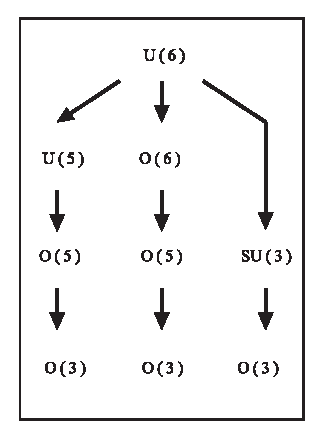
\includegraphics[height=4cm]{figure.eps}
%
% If not, use
%\picplace{5cm}{2cm} % Give the correct figure height and width in cm
%
\caption{Please write your figure caption here}
\label{fig:1}       % Give a unique label
\end{figure}
%
% For built-in environments use
%
\begin{theorem}
Theorem text goes here.
\end{theorem}
%
% or
%
\begin{lemma}
Lemma text goes here.
\end{lemma}
%
%
% Problems or Exercises should be sorted chapterwise
\section*{Problems}
\addcontentsline{toc}{section}{Problems}
%
% Use the following environment.
% Don't forget to label each problem;
% the label is needed for the solutions' environment
\begin{prob}
\label{prob1}
The problem\footnote{Footnote} is described here. The
problem is described here. The problem is described here.
\end{prob}

\begin{prob}
\label{prob2}
\textbf{Problem Heading}\\
(a) The first part of the problem is described here.\\
(b) The second part of the problem is described here.
\end{prob}



%

%!TEX root = book.tex

\chapter{Giới thiệu}
\label{cha:introduce}



Những năm gần đây, AI - Artificial Intelligence (Trí Tuệ Nhân Tạo), và cụ thể hơn là Machine Learning (Học Máy hoặc Máy Học - {\it Với những từ chuyên ngành, tôi sẽ dùng song song cả tiếng Anh và tiếng Việt, tuy nhiên sẽ ưu tiên tiếng Anh vì thuận tiện hơn trong việc tra cứu}) nổi lên như một bằng chứng của cuộc cách mạng công nghiệp lần thứ tư (1 - động cơ hơi nước, 2 - năng lượng điện, 3 - công nghệ thông tin). Trí Tuệ Nhân Tạo đang len lỏi vào mọi lĩnh vực trong đời sống mà có thể chúng ta không nhận ra. Xe tự hành của Google và Tesla, hệ thống tự tag khuôn mặt trong ảnh của Facebook, trợ lý ảo Siri của Apple, hệ thống gợi ý sản phẩm của Amazon, hệ thống gợi ý phim của Netflix, máy chơi cờ vây AlphaGo của Google DeepMind, ..., chỉ là một vài trong vô vàn những ứng dụng của AI/Machine Learning. (Xem thêm \href{{https://www.facebook.com/zuck/posts/10103351073024591}}{Jarvis - trợ lý thông minh cho căn nhà của Mark Zuckerberg}.)

% \url{https://www.facebook.com/zuck/posts/10103351073024591}


Machine Learning là một tập con của AI. Theo định nghĩa của Wikipedia, {\it Machine learning is the subfield of computer science that "gives computers the ability to learn without being explicitly programmed"}. Nói đơn giản, Machine Learning là một lĩnh vực nhỏ của Khoa Học Máy Tính, nó có khả năng tự học hỏi dựa trên dữ liệu đưa vào mà không cần phải được lập trình cụ thể. Bạn Nguyễn Xuân Khánh tại đại học Maryland đang viết một cuốn sách về Machine Learning bằng tiếng Việt khá thú vị, các bạn có thể tham khảo bài \href{https://ml-book-vn.khanhxnguyen.com/intro.html}{Machine Learning là gì?}.

Những năm gần đây, {khi mà khả năng tính toán} của các máy tính được nâng lên một tầm cao mới và lượng dữ liệu khổng lồ được thu thập bởi các hãng công nghệ lớn, Machine Learning đã tiến thêm một bước tiến dài và một lĩnh vực mới được ra đời gọi là Deep Learning (Học Sâu). Deep Learning đã giúp máy tính thực thi những việc tưởng chừng như không thể vào 10 năm trước: phân loại cả ngàn vật thể khác nhau trong các bức ảnh, tự tạo chú thích cho ảnh, bắt chước giọng nói và chữ viết của con người, giao tiếp với con người, hay thậm chí cả sáng tác văn hay âm nhạc (Xem thêm \href{{http://machinelearningmastery.com/inspirational-applications-deep-learning/}}{8 Inspirational Applications of Deep Learning}).

Mối quan hệ giữa Artificial Intelligence, Machine Learning, và Deep Learning được cho trong Hình \ref{fig:aimldl}.

\begin{figure}
\centering
	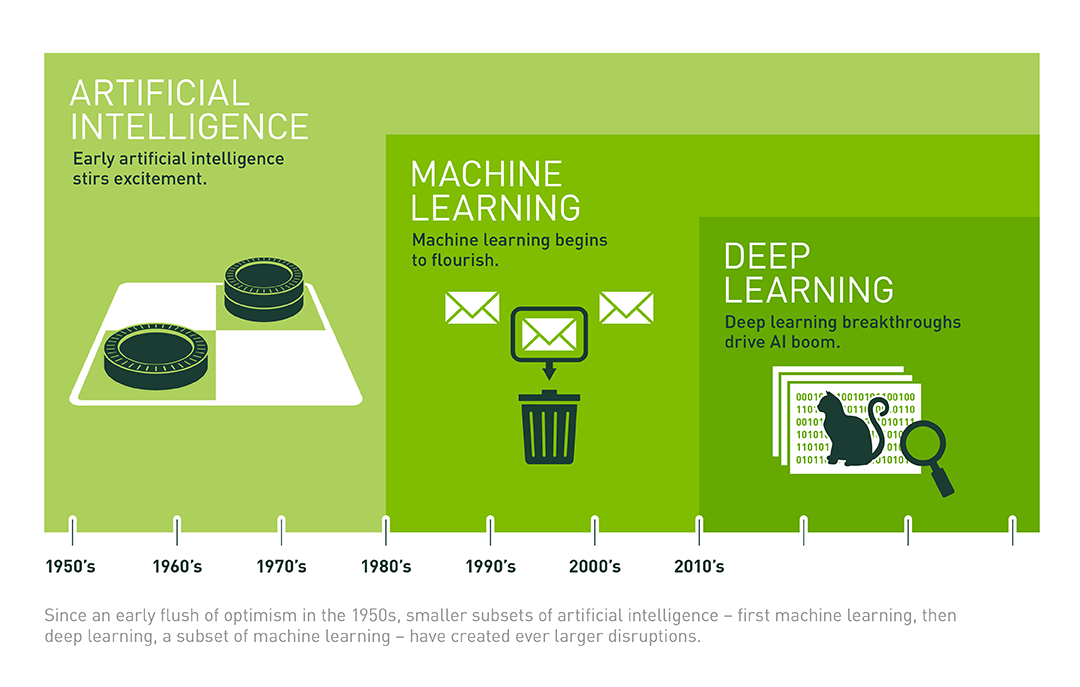
\includegraphics[width = \textwidth]{../introduce/aimldl.png}
	\caption[]{Mối quan hệ giữa AI, Machine Learning và Deep Learning. Nguồn: \href{https://blogs.nvidia.com/blog/2016/07/29/whats-difference-artificial-intelligence-machine-learning-deep-learning-ai/}{What’s the Difference Between Artificial Intelligence, Machine Learning, and Deep Learning?}}
	\label{fig:aimldl}
\end{figure}

% <div class="imgcap">
% <div >
%     <img src="/assets/introduce/aimldl.png" width = "800"></a>
%     <!-- <img src="/assets/rl/mdp.png" height="206"> -->
% </div>
% <div class="thecap">Mối quan hệ giữa AI, Machine Learning và Deep Learning. <br> (Nguồn: <a href="https://blogs.nvidia.com/blog/2016/07/29/whats-difference-artificial-intelligence-machine-learning-deep-learning-ai/">What’s the Difference Between Artificial Intelligence, Machine Learning, and Deep Learning?</a>)</div>
% </div>

\section{Mục đích viết Blog}
Nhu cầu về nhân lực ngành Machine Learning (Deep Learning) đang ngày một cao, kéo theo đó nhu cầu học Machine Learning trên thế giới và ở Việt Nam ngày một lớn. Cá nhân tôi cũng muốn hệ thống lại kiến thức của mình về lĩnh vực này để chuẩn bị cho tương lai (đây là một trong những mục tiêu của tôi trong năm 2017). Tôi sẽ cố gắng đi từ những thuật toán cơ bản nhất của Machine Learning kèm theo các ví dụ và mã nguồn trong mỗi bài viết. Tôi sẽ viết 1-2 tuần 1 bài (việc viết các công thức toán và code trên blog thực sự tốn nhiều thời gian hơn tôi từng nghĩ). Đồng thơi, tôi cũng mong muốn nhận được phản hồi của bạn đọc để qua những thảo luận, tôi và các bạn có thể nắm bắt được các thuật toán này. 

Khi chuẩn bị các bài viết, tôi sẽ giả định rằng bạn đọc có một chút kiến thức về Đại Số Tuyến Tính (Linear Algebra), Xác Suât Thống Kê (Probability and Statistics) và có kinh nghiệm về lập trình Python. Nếu bạn chưa có nhiều kinh nghiệm về các lĩnh vực này, đừng quá lo lắng vì mỗi bài sẽ chỉ sử dụng một vài kỹ thuật cơ bản. Hãy để lại câu hỏi của bạn ở phần Comment bên dưới mỗi bài, tôi sẽ thảo luận thêm với các bạn.

Trong bài tiếp theo của blog này, tôi sẽ giới thiệu về các nhóm thuật toán Machine learning cơ bản. Mời các bạn theo dõi. 

\section{Tham khảo thêm}
\subsection{Các khóa học}
\subsubsection{Tiếng Anh}
\begin{enumerate}
	\item \href{https://www.coursera.org/learn/machine-learning}{Machine Learning với thầy Andrew Ng trên Coursera} ({\it Khóa học nổi tiếng nhất về Machine Learning })

	\item \href{https://www.udacity.com/course/deep-learning--ud730}{Deep Learning by Google trên Udacity} ({\it Khóa học nâng cao hơn về Deep Learning với Tensorflow})


	\item \href{http://machinelearningmastery.com/}{Machine Learning mastery} ({\it Các thuật toán Machine Learning cơ bản})
\end{enumerate}

\subsubsection{Tiếng Việt}
{\bf Lưu ý}: {\it Các khóa học này tôi chưa từng tham gia, chỉ đưa ra để các bạn tham khảo.}
\begin{enumerate}
	\item \href{http://tuanvannguyen.blogspot.com/2016/12/cap-nhat-khoa-hoc-ve-machine-learning.html}{Machine Learning 1/2017}


	\item \href{https://techmaster.vn/khoa-hoc/25511/machine-learning-co-ban}{Nhập môn Machine Learning, Tech Master- Cao Thanh Hà {\it POSTECH}}() 

\end{enumerate}

\subsection{Các trang Machine Learning tiếng Việt khác}
\begin{enumerate}
	\item \href{http://viet.jnlp.org/kien-thuc-co-ban-ve-xu-ly-ngon-ngu-tu-nhien/machine-learning-trong-nlp}{Machine Learning trong Xử Lý Ngôn Ngữ Tự Nhiên - Nhóm Đông Du {\it Nhật Bản}}

	\item \href{https://ongxuanhong.wordpress.com/}{Machine Learning cho người mới bắt đầu - Ông Xuân Hồng {\it JAIST}}. 

	
	 \item \href{https://ml-book-vn.khanhxnguyen.com/}{Machine Learning book for Vietnamese - Nguyễn Xuân Khánh \textit{University of Maryland}}
\end{enumerate}
% 3. [Machine Learning trong Xử Lý Ngôn Ngữ Tự Nhiên - Nhóm Đông Du _Nhật Bản_](http://viet.jnlp.org/kien-thuc-co-ban-ve-xu-ly-ngon-ngu-tu-nhien/machine-learning-trong-nlp)
% 4. [Machine Learning cho người mới bắt đầu - Ông Xuân Hồng _JAIST_](https://ongxuanhong.wordpress.com/). 
% 5. [Machine Learning book for Vietnamese - Nguyễn Xuân Khánh _University of Maryland_](https://ml-book-vn.khanhxnguyen.com/)
%!TEX root = ML_book.tex
\chapter{Phân nhóm các thuật toán Machine Learning}

Có hai cách phổ biến phân nhóm các thuật toán Machine learning. Một là dựa trên phương thức học (learning style), hai là dựa trên chức năng (function) (của mỗi thuật toán).

%!TEX root = book.tex
\chapter{Linear Regression }

 
Trong bài này, tôi sẽ giới thiệu một trong những thuật toán cơ bản nhất (và đơn giản nhất) của Machine Learning. Đây là một thuật toán \textit{Supervised learning} có tên \textbf{Linear Regression} (Hồi Quy Tuyến Tính). Bài toán này đôi khi được gọi là \textit{Linear Fitting} (trong thống kê) hoặc \textit{Linear Least Square}. 

\section{Giới thiệu}
 
Quay lại \href{http://machinelearningcoban.com/2016/12/27/categories/#regression-hoi-quy}{ví dụ đơn giản được nêu trong bài trước}: một căn nhà rộng $x_1 ~ \text{m}^2$, có $x_2$ phòng ngủ và cách trung tâm thành phố $x_3~ \text{km}$ có giá là bao nhiêu. Giả sử chúng ta đã có số liệu thống kê từ 1000 căn nhà trong thành phố đó, liệu rằng khi có một căn nhà mới với các thông số về diện tích, số phòng ngủ và khoảng cách tới trung tâm, chúng ta có thể dự đoán được giá của căn nhà đó không? Nếu có thì hàm dự đoán $y = f(\mathbf{x}) $ sẽ có dạng như thế nào. Ở đây $\mathbf{x} = [x_1, x_2, x_3] $ là một vector hàng chứa thông tin \textit{input}, $y$ là một số vô hướng (scalar) biểu diễn \textit{output} (tức giá của căn nhà trong ví dụ này). 
 
\textbf{Lưu ý về ký hiệu toán học:} \textit{trong các bài viết của tôi, các số vô hướng được biểu diễn bởi các chữ cái viết ở dạng không in đậm, có thể viết hoa, ví dụ $x_1, N, y, k$. Các vector được biểu diễn bằng các chữ cái thường in đậm, ví dụ $\mathbf{y}, \mathbf{x}_1 $. Các ma trận được biểu diễn bởi các chữ viết hoa in đậm, ví dụ $\mathbf{X, Y, W} $.} 
 
Một cách đơn giản nhất, chúng ta có thể thấy rằng: i) diện tích nhà càng lớn thì giá nhà càng cao; ii) số lượng phòng ngủ càng lớn thì giá nhà càng cao; iii) càng xa trung tâm thì giá nhà càng giảm. Một hàm số đơn giản nhất có thể mô tả mối quan hệ giữa giá nhà và 3 đại lượng đầu vào là:  
 
 
$$y \approx  f(\mathbf{x}) = \hat{y}$$ 
$$f(\mathbf{x}) =w_1 x_1 + w_2 x_2 + w_3 x_3 + w_0 ~~~~ (1)$$ 
trong đó, $w_1, w_2, w_3, w_0$ là các hằng số,  $w_0$ còn được gọi là bias. Mối quan hệ $y \approx f(\mathbf{x})$ bên trên là một mối quan hệ tuyến tính (linear). Bài toán chúng ta đang làm là một bài toán thuộc loại regression. Bài toán đi tìm các hệ số tối ưu $ \\{w_1, w_2, w_3, w_0 \\}$ chính vì vậy được gọi là bài toán Linear Regression.  
 
\textbf{Chú ý 1:} $y$ là giá trị thực của \textit{outcome} (dựa trên số liệu thống kê chúng ta có trong tập \textit{training data}), trong khi $\hat{y}$ là giá trị mà mô hình Linear Regression dự đoán được. Nhìn chung, $y$ và $\hat{y}$ là hai giá trị khác nhau do có sai số mô hình, tuy nhiên, chúng ta mong muốn rằng sự khác nhau này rất nhỏ. 
 
\textbf{Chú ý 2:} \textit{Linear} hay \textit{tuyến tính} hiểu một cách đơn giản là \textit{thẳng, phẳng}. Trong không gian hai chiều, một hàm số được gọi là \textit{tuyến tính} nếu đồ thị của nó có dạng một \textit{đường thẳng}. Trong không gian ba chiều, một hàm số được goi là \textit{tuyến tính} nếu đồ thị của nó có dạng một \textit{mặt phẳng}. Trong không gian nhiều hơn 3 chiều, khái niệm \textit{mặt phẳng} không còn phù hợp nữa, thay vào đó, một khái niệm khác ra đời được gọi là \textit{siêu mặt phẳng} (\textit{hyperplane}). Các hàm số tuyến tính là các hàm đơn giản nhất, vì chúng thuận tiện trong việc hình dung và tính toán. Chúng ta sẽ được thấy trong các bài viết sau, \textit{tuyến tính} rất quan trọng và hữu ích trong các bài toán Machine Learning. Kinh nghiệm cá nhân tôi cho thấy, trước khi hiểu được các thuật toán \textit{phi tuyến} (non-linear, không phẳng), chúng ta cần nắm vững các kỹ thuật cho các mô hình \textit{tuyến tính}. 
 
 
 
 
 
\section{Phân tích toán học}
 
 
 
 
\subsection{Dạng của Linear Regression }
 
Trong phương trình $(1)$ phía trên, nếu chúng ta đặt $\mathbf{w} = [w_0, w_1, w_2, w_3]^T = $ là vector (cột) hệ số cần phải tối ưu và $\mathbf{\bar{x}} = [1, x_1, x_2, x_3]$ (đọc là \textit{x bar} trong tiếng Anh) là vector (hàng) dữ liệu đầu vào \textit{mở rộng}. Số $1$ ở đầu được thêm vào để phép tính đơn giản hơn và thuận tiện cho việc tính toán. Khi đó, phương trình (1) có thể được viết lại dưới dạng: 
 
$$y \approx \mathbf{\bar{x}}\mathbf{w} = \hat{y}$$ 
 
Chú ý rằng $\mathbf{\bar{x}}$ là một vector hàng. (\href{http://machinelearningcoban.com/math/#luu-y-ve-ky-hieu}{Xem thêm về ký hiệu vector hàng và cột tại đây}) 
 
 
 
\subsection{Sai số dự đoán }
 
Chúng ta mong muốn rằng sự sai khác $e$ giữa giá trị thực $y$ và giá trị dự đoán $\hat{y}$ (đọc là \textit{y hat} trong tiếng Anh) là nhỏ nhất. Nói cách khác, chúng ta muốn giá trị sau đây càng nhỏ càng tốt:  
 
$$ 
\frac{1}{2}e^2 = \frac{1}{2}(y - \hat{y})^2 = \frac{1}{2}(y - \mathbf{\bar{x}}\mathbf{w})^2 
$$ 
 
trong đó hệ số $\frac{1}{2} $ (\textit{lại}) là để thuận tiện cho việc tính toán (khi tính đạo hàm thì số $\frac{1}{2} $ sẽ bị triệt tiêu). Chúng ta cần $e^2$ vì $e = y - \hat{y} $ có thể là một số âm, việc nói $e$ nhỏ nhất sẽ không đúng vì khi $e = - \infty$ là rất nhỏ nhưng sự sai lệch là rất lớn. Bạn đọc có thể tự đặt câu hỏi: \textbf{tại sao không dùng trị tuyệt đối $ \|e\| $ mà lại dùng bình phương $e^2$ ở đây?} Câu trả lời sẽ có ở phần sau.  
 
 
 
 
 
 
\subsection{Hàm mất mát}
 
Điều tương tự xảy ra với tất cả các cặp \textit{(input, outcome)} $ (\mathbf{x}_i, y_i), i = 1, 2, \dots, N $, với $N$ là số lượng dữ liệu quan sát được. Điều chúng ta muốn, tổng sai số là nhỏ nhất, tương đương với việc tìm $ \mathbf{w} $ để hàm số sau đạt giá trị nhỏ nhất: 
 
$$ \mathcal{L}(\mathbf{w}) = \frac{1}{2}\sum_{i=1}^N (y_i - \mathbf{\bar{x}_i}\mathbf{w})^2 ~~~~~(2) $$  
 
Hàm số $\mathcal{L}(\mathbf{w}) $ được gọi là \textbf{hàm mất mát} (loss function) của bài toán Linear Regression. Chúng ta luôn mong muốn rằng sự mất mát (sai số) là nhỏ nhất, điều đó đồng nghĩa với việc  tìm vector hệ số $ \mathbf{w} $  sao cho  
giá trị của hàm mất mát này càng nhỏ càng tốt. Giá trị của $\mathbf{w}$ làm cho hàm mất mát đạt giá trị nhỏ nhất được gọi là \textit{điểm tối ưu} (optimal point), ký hiệu: 
 
$$ \mathbf{w}^* = \arg\min_{\mathbf{w}} \mathcal{L}(\mathbf{w})  $$  
 
Trước khi đi tìm lời giải, chúng ta đơn giản hóa phép toán trong phương trình hàm mất mát $(2)$. Đặt $\mathbf{y} = [y_1; y_2; \dots; y_N]$ là một vector cột chứa tất cả các \textit{output} của \textit{training data}; $ \mathbf{\bar{X}} = [\mathbf{\bar{x}}_1; \mathbf{\bar{x}}_2; \dots; \mathbf{\bar{x}}_N ] $ là ma trận dữ liệu đầu vào (mở rộng) mà mỗi hàng của nó là một điểm dữ liệu. Khi đó hàm số mất mát $\mathcal{L}(\mathbf{w})$ được viết dưới dạng ma trận đơn giản hơn: 
 
$$ 
\mathcal{L}(\mathbf{w})  
= \frac{1}{2}\sum_{i=1}^N (y_i - \mathbf{\bar{x}}_i\mathbf{w})^2 $$ 
$$ 
= \frac{1}{2} \|\mathbf{y} - \mathbf{\bar{X}}\mathbf{w} \|_2^2  
~~~(3) 
$$ 
 
với $ \| \mathbf{z} \|_2 $ là Euclidean norm (chuẩn Euclid, hay khoảng cách Euclid), nói cách khác $ \| \mathbf{z} \|_2^2 $ là tổng của bình phương mỗi phần tử của vector $\mathbf{z}$. Tới đây, ta đã có một dạng đơn giản của hàm mất mát được viết như phương trình $(3)$. 
 
 
 
 
 
\subsection{Nghiệm cho bài toán Linear Regression}
 
\textbf{Cách phổ biến nhất để tìm nghiệm cho một bài toán tối ưu (chúng ta đã biết từ khi học cấp 3) là giải phương trình đạo hàm (gradient) bằng 0!} Tất nhiên đó là khi việc tính đạo hàm và việc giải phương trình đạo hàm bằng 0 không quá phức tạp. Thật may mắn, với các mô hình tuyến tính, hai việc này là khả thi.  
 
Đạo hàm theo $\mathbf{w} $ của hàm mất mát là:  
$$ 
\frac{\partial{\mathcal{L}(\mathbf{w})}}{\partial{\mathbf{w}}}  
= \mathbf{\bar{X}}^T(\mathbf{\bar{X}}\mathbf{w} - \mathbf{y})  
$$ 
 
Các bạn có thể tham khảo bảng đạo hàm theo vector hoặc ma trận của một hàm số trong \href{https://ccrma.stanford.edu/~dattorro/matrixcalc.pdf}{mục D.2 của tài liệu này}. \textit{Đến đây tôi xin quay lại câu hỏi ở phần Sai số dự đoán phía trên về việc tại sao không dùng trị tuyệt đối mà lại dùng bình phương. Câu trả lời là hàm bình phương có đạo hàm tại mọi nơi, trong khi hàm trị tuyệt đối thì không (đạo hàm không xác định tại 0)}. 
 
Phương trình đạo hàm bằng 0 tương đương với:  
$$ 
\mathbf{\bar{X}}^T\mathbf{\bar{X}}\mathbf{w} = \mathbf{\bar{X}}^T\mathbf{y} \triangleq \mathbf{b}  
~~~ (4) 
$$ 
(ký hiệu $\mathbf{\bar{X}}^T\mathbf{y} \triangleq \mathbf{b} $ nghĩa là \textit{đặt} $\mathbf{\bar{X}}^T\mathbf{y}$ \textit{bằng} $\mathbf{b}$ ). 
 
Nếu ma trận vuông $ \mathbf{A} \triangleq \mathbf{\bar{X}}^T\mathbf{\bar{X}}$ khả nghịch (non-singular hay inversable) thì phương trình $(4)$ có nghiệm duy nhất: $ \mathbf{w} = \mathbf{A}^{-1}\mathbf{b}  $. 
 
Vậy nếu ma trận $\mathbf{A} $ không khả nghịch (có định thức bằng 0) thì sao? Nếu các bạn vẫn nhớ các kiến thức về hệ phương trình tuyến tính, trong trường hợp này thì hoặc phương trinh $ (4) $ vô nghiệm, hoặc làp  
nó 
có vô số nghiệm. Khi đó, chúng ta sử dụng khái niệm \href{https://vi.wikipedia.org/wiki/Giả_nghịch_đảo_Moore–Penrose}{\textit{giả nghịch đảo}} $ \mathbf{A}^{\dagger} $ (đọc là \textit{A dagger} trong tiếng Anh). (\textit{Giả nghịch đảo (pseudo inverse) là trường hợp tổng quát của nghịch đảo khi ma trận không khả nghịch hoặc thậm chí không vuông. Trong khuôn khổ bài viết này, tôi xin phép được lược bỏ phần này, nếu các bạn thực sự quan tâm, tôi sẽ viết một bài khác chỉ nói về giả nghịch đảo. Xem thêm: \href{http://www.sci.utah.edu/~gerig/CS6640-F2012/Materials/pseudoinverse-cis61009sl10.pdf}{Least Squares, Pseudo-Inverses, PCA \& SVD}.}) 
 
Với khái niệm giả nghịch đảo, điểm tối ưu của bài toán Linear Regression có dạng: 
 
 
$$ 
\mathbf{w} = \mathbf{A}^{\dagger}\mathbf{b} = (\mathbf{\bar{X}}^T\mathbf{\bar{X}})^{\dagger} \mathbf{\bar{X}}^T\mathbf{y} 
~~~ (5) 
$$ 
 
 
 
 
\section{Ví dụ trên Python}
 
 
\subsection{Bài toán}
 
Trong phần này, tôi sẽ chọn một ví dụ đơn giản về việc giải bài toán Linear Regression trong Python. Tôi cũng sẽ so sánh nghiệm của bài toán khi giải theo phương trình $(5) $ và nghiệm tìm được khi dùng thư viện \href{http://scikit-learn.org/stable/}{scikit-learn} của Python. (\textit{Đây là thư viện Machine Learning được sử dụng rộng rãi trong Python}). Trong ví dụ này, dữ liệu đầu vào chỉ có 1 giá trị (1 chiều) để thuận tiện cho việc minh hoạ trong mặt phẳng.  
 
Chúng ta có 1 bảng dữ liệu về chiều cao và cân nặng của 15 người như dưới đây: 
 
 
| Chiều cao (cm)     | Cân nặng (km)     | Chiều cao (cm)     | Cân nặng (kg)     | 
| :----------------: | :---------------: | :----------------: | :---------------: | 
| 147                | 49                | 168                | 60                | 
| 150                | 50                | 170                | 72                | 
| 153                | 51                | 173                | 63                | 
| 155                | 52                | 175                | 64                | 
| 158                | 54                | 178                | 66                | 
| 160                | 56                | 180                | 67                | 
| 163                | 58                | 183                | 68                | 
| 165                | 59                |                    |                   | 
 
 
Bài toán đặt ra là: liệu có thể dự đoán cân nặng của một người dựa vào chiều cao của họ không? (\textit{Trên thực tế, tất nhiên là không, vì cân nặng còn phụ thuộc vào nhiều yếu tố khác nữa, thể tích chẳng hạn}). Vì blog này nói về các thuật toán Machine Learning đơn giản nên tôi sẽ giả sử rằng chúng ta có thể dự đoán được. 
 
Chúng ta có thể thấy là cân nặng sẽ tỉ lệ thuận với chiều cao (càng cao càng nặng), nên có thể sử dụng Linear Regression model cho việc dự đoán này. Để kiểm tra độ chính xác của model tìm được, chúng ta sẽ giữ lại cột 155 và 160 cm để kiểm thử, các cột còn lại được sử dụng để huấn luyện (train) model. 
 
 
\subsection{Hiển thị dữ liệu trên đồ thị}
Trước tiên, chúng ta cần có hai thư viện \href{http://www.numpy.org/}{numpy} cho đại số tuyến tính và \href{http://matplotlib.org/}{matplotlib} cho việc vẽ hình.  
 
 
\begin{lstlisting}[language=Python]
# To support both python 2 and python 3 
from __future__ import division, print_function, unicode_literals 
import numpy as np  
import matplotlib.pyplot as plt 
\end{lstlisting}
 
Tiếp theo, chúng ta khai báo và biểu diễn dữ liệu trên một đồ thị. 
 
 
\begin{lstlisting}[language=Python]
# height (cm) 
X = np.array([[147, 150, 153, 158, 163, 165, 168, 170, 173, 175, 178, 180, 183]]).T 
# weight (kg) 
y = np.array([[ 49, 50, 51,  54, 58, 59, 60, 62, 63, 64, 66, 67, 68]]).T 
# Visualize data  
plt.plot(X, y, 'ro') 
plt.axis([140, 190, 45, 75]) 
plt.xlabel('Height (cm)') 
plt.ylabel('Weight (kg)') 
plt.show() 
\end{lstlisting}
 
 
% <div class="imgcap"> 
% <img src ="/assets/LR/output_3_0.png" align = "center"> 
% </div> 
 
 \begin{figure}
 	\centering	
 	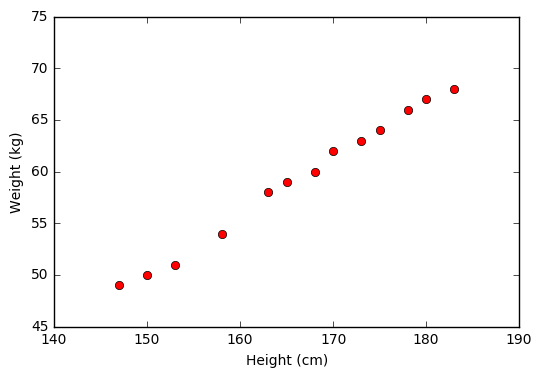
\includegraphics[width = \textwidth]{../LR/output_3_0.png}
 \end{figure}
 
Từ đồ thị này ta thấy rằng dữ liệu được sắp xếp gần như theo 1 đường thẳng, vậy mô hình Linear Regression nhiều khả năng sẽ cho kết quả tốt: 
 
(cân nặng) = \pythoninline{w\_1}*(chiều cao) + \pythoninline{w\_0} 
 
 
\subsection{Nghiệm theo công thức}
 
Tiếp theo, chúng ta sẽ tính toán các hệ số \pythoninline{w_1} và \pythoninline{w_0} dựa vào công thức $(5)$. Chú ý: giả nghịch đảo của một ma trận \pythoninline{A} trong Python sẽ được tính bằng \pythoninline{numpy.linalg.pinv(A)}, \pythoninline{pinv} là từ viết tắt của \textit{pseudo inverse}. 
 
\begin{lstlisting}[language=Python]
# Building Xbar  
one = np.ones((X.shape[0], 1)) 
Xbar = np.concatenate((one, X), axis = 1) 
 
# Calculating weights of the fitting line  
A = np.dot(Xbar.T, Xbar) 
b = np.dot(Xbar.T, y) 
w = np.dot(np.linalg.pinv(A), b) 
print('w = ', w) 
# Preparing the fitting line  
w_0 = w[0][0] 
w_1 = w[1][0] 
x0 = np.linspace(145, 185, 2) 
y0 = w_0 + w_1*x0 
 
# Drawing the fitting line  
plt.plot(X.T, y.T, 'ro')     # data  
plt.plot(x0, y0)               # the fitting line 
plt.axis([140, 190, 45, 75]) 
plt.xlabel('Height (cm)') 
plt.ylabel('Weight (kg)') 
plt.show() 
 
\end{lstlisting}
 
\begin{lstlisting}[language=Python]
w =  [[-33.73541021] 
 [  0.55920496]] 
\end{lstlisting}
 
 


\begin{figure}
	\centering
	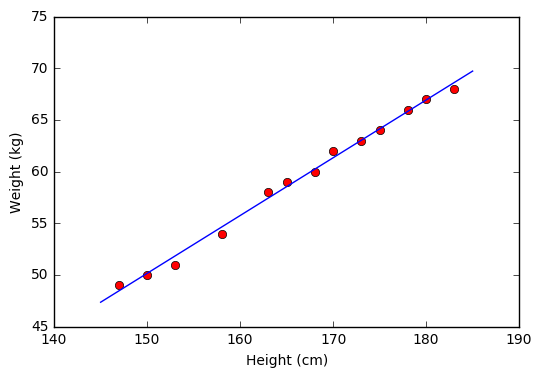
\includegraphics[width = \textwidth]{../LR/output_5_1.png}
\end{figure}
 
Từ đồ thị bên trên ta thấy rằng các điểm dữ liệu màu đỏ nằm khá gần đường thẳng dự đoán màu xanh. Vậy mô hình Linear Regression hoạt động tốt với tập dữ liệu \textit{training}. Bây giờ, chúng ta sử dụng mô hình này để dự đoán cân nặng của hai người có chiều cao 155 và 160 cm mà chúng ta đã không dùng khi tính toán nghiệm. 
 
 
\begin{lstlisting}[language=Python]
y1 = w_1*155 + w_0 
y2 = w_1*160 + w_0 
 
print( 'Predict weight of person with height 155 cm: %.2f (kg), real number: 52 (kg)'  %(y1) ) 
print( 'Predict weight of person with height 160 cm: %.2f (kg), real number: 56 (kg)'  %(y2) ) 
\end{lstlisting}
 
    Predict weight of person with height 155 cm: 52.94 (kg), real number: 52 (kg) 
    Predict weight of person with height 160 cm: 55.74 (kg), real number: 56 (kg) 
 
 
 
Chúng ta thấy rằng kết quả dự đoán khá gần với số liệu thực tế. 
 
 
\subsection{Nghiệm theo thư viện scikit-learn}
 
Tiếp theo, chúng ta sẽ sử dụng thư viện scikit-learn của Python để tìm nghiệm.  
 
 
\begin{lstlisting}[language=Python]
from sklearn import datasets, linear_model 
 
# fit the model by Linear Regression 
regr = linear_model.LinearRegression(fit_intercept=False) # fit_intercept = False for calculating the bias 
regr.fit(Xbar, y) 
 
# Compare two results 
print( 'Solution found by scikit-learn  : ', regr.coef_ ) 
print( 'Solution found by (5): ', w.T) 
\end{lstlisting}
 
\begin{lstlisting}[language=Python]
    Solution found by scikit-learn  :  [[  -33.73541021 0.55920496]] 
    Solution found by (5):  [[  -33.73541021 0.55920496 ]] 
\end{lstlisting}
 
Chúng ta thấy rằng hai kết quả thu được như nhau! (\textit{Nghĩa là tôi đã không mắc lỗi nào trong cách tìm nghiệm ở phần trên}) 
 
\href{https://github.com/tiepvupsu/tiepvupsu.github.io/blob/master/assets/LR/LR.ipynb}{Source code Jupyter Notebook cho bài này.} 
 
 
 
\section{Thảo luận}
 
 
\subsection{Các bài toán có thể giải bằng Linear Regression}
Hàm số $y \approx f(\mathbf{x})= \mathbf{w}^T\mathbf{x}$ là một hàm tuyến tính theo cả $ \mathbf{w}$ và $\mathbf{x}$. Trên thực tế, Linear Regression có thể áp dụng cho các mô hình chỉ cần tuyến tính theo $\mathbf{w}$. Ví dụ: 
$$ 
y \approx w_1 x_1 + w_2 x_2 + w_3 x_1^2 +  w_4 \sin(x_2) + w_5 x_1x_2 + w_0 
$$ 
là một hàm tuyến tính theo $\mathbf{w}$ và vì vậy cũng có thể được giải bằng Linear Regression. Với mỗi dữ liệu đầu vào $\mathbf{x}=[x_1; x_2] $, chúng ta tính toán dữ liệu mới $\tilde{\mathbf{x}} = [x_1, x_2, x_1^2, \sin(x_2), x_1x_2]$ (đọc là \textit{x tilde} trong tiếng Anh) rồi áp dụng Linear Regression với dữ liệu mới này.  
 
Xem thêm ví dụ về \href{http://www.varsitytutors.com/hotmath/hotmath_help/topics/quadratic-regression}{Quadratic Regression} (Hồi Quy Bậc Hai). 
% <div class="imgcap"> 
% <div > 
%     <img src ="http://www.varsitytutors.com/assets/vt-hotmath-legacy/hotmath_help/topics/quadratic-regression/f-qr-1-1.gif"  width = "300"></a> 
% </div> 
% <div class="thecap"> Quadratic Regression (Nguồn: <a href = "http://www.varsitytutors.com/hotmath/hotmath_help/topics/quadratic-regression"> Quadratic Regression</a>) <br></div> 
% </div> 
 
 a figre should be here 
 
\subsection{Hạn chế của Linear Regression}
 
Hạn chế đầu tiên của Linear Regression là nó rất \textbf{nhạy cảm với nhiễu} (sensitive to noise). Trong ví dụ về mối quan hệ giữa chiều cao và cân nặng bên trên, nếu có chỉ 
một cặp dữ liệu \textit{nhiễu} (150 cm, 90kg) thì kết quả sẽ sai khác đi rất nhiều. Xem hình dưới đây: 
% <div class="imgcap"> 
% <img src ="/assets/LR/output_13_1.png" align = "center"> 
% </div> 
 
 \begin{figure}
 	\centering
 	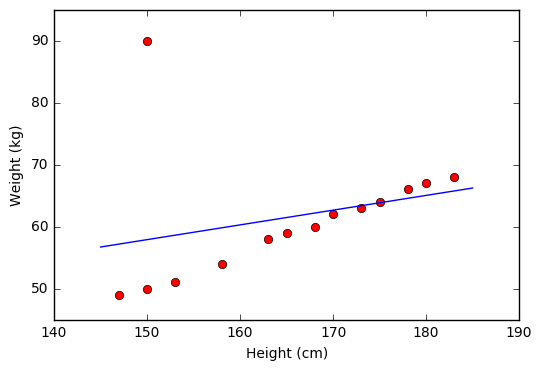
\includegraphics[width = .6\textwidth]{../LR/output_13_1.png}
 \end{figure}
Vì vậy, trước khi thực hiện Linear Regression, các nhiễu (\textit{outlier}) cần 
 phải được loại bỏ. Bước này được gọi là tiền xử lý (pre-processing). 
 
Hạn chế thứ hai của Linear Regression là nó \textbf{không biễu diễn được các mô hình phức tạp}. Mặc dù trong phần trên, chúng ta thấy rằng phương pháp này có thể được áp dụng nếu quan hệ giữa \textit{outcome} và \textit{input} không nhất thiết phải là tuyến tính, nhưng mối quan hệ này vẫn đơn giản nhiều so với các mô hình thực tế. Hơn nữa, chúng ta sẽ tự hỏi: làm thế nào để xác định được các hàm $x_1^2, \sin(x_2), x_1x_2$ như ở trên?! 
 
 
\subsection{Các phương pháp tối ưu}
Linear Regression là một mô hình đơn giản, lời giải cho phương trình đạo hàm bằng 0 cũng khá đơn giản. \textit{Trong hầu hết các trường hợp, chúng ta không thể giải được phương trình đạo hàm bằng 0.} 
 
Nhưng có một điều chúng ta nên nhớ, \textbf{còn tính được đạo hàm là còn có cơ hội}. 
 
 
 
 
\section{Tài liệu tham khảo}
 
1. \href{https://en.wikipedia.org/wiki/Linear_regression}{Linear Regression - Wikipedia} 
2. \href{http://machinelearningmastery.com/simple-linear-regression-tutorial-for-machine-learning/}{Simple Linear Regression Tutorial for Machine Learning} 
3. \href{http://www.sci.utah.edu/~gerig/CS6640-F2012/Materials/pseudoinverse-cis61009sl10.pdf}{Least Squares, Pseudo-Inverses, PCA \& SVD} 



\begin{lstlisting}[language=Python, caption=Python example]
import numpy as np
 
def incmatrix(genl1,genl2):
    m = len(genl1)
    n = len(genl2)
    M = None #to become the incidence matrix
    VT = np.zeros((n*m,1), int)  #dummy variable
 
    #compute the bitwise xor matrix
    M1 = bitxormatrix(genl1)
    M2 = np.triu(bitxormatrix(genl2),1) 
 
    for i in range(m-1):
        for j in range(i+1, m):
            [r,c] = np.where(M2 == M1[i,j])
            for k in range(len(r)):
                VT[(i)*n + r[k]] = 1;
                VT[(i)*n + c[k]] = 1;
                VT[(j)*n + r[k]] = 1;
                VT[(j)*n + c[k]] = 1;
 
                if M is None:
                    M = np.copy(VT)
                else:
                    M = np.concatenate((M, VT), 1)
 
                VT = np.zeros((n*m,1), int)
 
    return M
\end{lstlisting}


%%%%%%%%%%%%%%%%%%%%%% chapter.tex %%%%%%%%%%%%%%%%%%%%%%%%%%%%%%%%%
%
% sample chapter
%
% Use this file as a template for your own input.
%
%%%%%%%%%%%%%%%%%%%%%%%% Springer-Verlag %%%%%%%%%%%%%%%%%%%%%%%%%%

\chapter{Linear Regression}
\label{intro} % Always give a unique label
% use \chaptermark{}
% to alter or adjust the chapter heading in the running head

Your text goes here. Separate text sections with the standard \LaTeX\
sectioning commands.

\section{Section Heading}
\label{sec:1}
% Always give a unique label
% and use \ref{<label>} for cross-references
% and \cite{<label>} for bibliographic references
% use \sectionmark{}
% to alter or adjust the section heading in the running head
Your text goes here. Use the \LaTeX\ automatism for your citations
\cite{monograph}.

\subsection{Subsection Heading}
\label{sec:2}
Your text goes here.

\begin{equation}
\vec{a}\times\vec{b}=\vec{c}
\end{equation}

\subsubsection{Subsubsection Heading}
Your text goes here. Use the \LaTeX\ automatism for cross-references as
well as for your citations, see Sect.~\ref{sec:1}.

\paragraph{Paragraph Heading} %
Your text goes here.

\subparagraph{Subparagraph Heading.} Your text goes here.%
%
\index{paragraph}
% Use the \index{} command to code your index words
%
% For tables use
%
\begin{table}
\centering
\caption{Please write your table caption here}
\label{tab:1}       % Give a unique label
%
% For LaTeX tables use
%
\begin{tabular}{lll}
\hline\noalign{\smallskip}
first & second & third  \\
\noalign{\smallskip}\hline\noalign{\smallskip}
number & number & number \\
number & number & number \\
\noalign{\smallskip}\hline
\end{tabular}
\end{table}
%
%
% For figures use
%
\begin{figure}
\centering
% Use the relevant command for your figure-insertion program
% to insert the figure file.
% For example, with the option graphics use
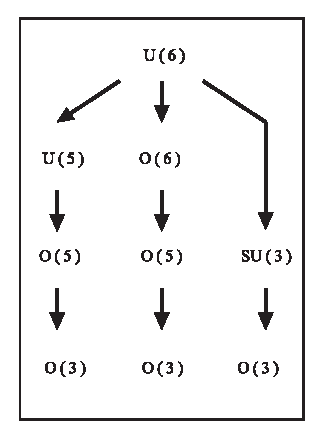
\includegraphics[height=4cm]{figure.eps}
%
% If not, use
%\picplace{5cm}{2cm} % Give the correct figure height and width in cm
%
\caption{Please write your figure caption here}
\label{fig:1}       % Give a unique label
\end{figure}
%
% For built-in environments use
%
\begin{theorem}
Theorem text goes here.
\end{theorem}
%
% or
%
\begin{lemma}
Lemma text goes here.
\end{lemma}
%
%
% Problems or Exercises should be sorted chapterwise
\section*{Problems}
\addcontentsline{toc}{section}{Problems}
%
% Use the following environment.
% Don't forget to label each problem;
% the label is needed for the solutions' environment
\begin{prob}
\label{prob1}
The problem\footnote{Footnote} is described here. The
problem is described here. The problem is described here.
\end{prob}

\begin{prob}
\label{prob2}
\textbf{Problem Heading}\\
(a) The first part of the problem is described here.\\
(b) The second part of the problem is described here.
\end{prob}



%

%\appendix
%\documentclass[12pt]{article}
\usepackage{amsmath}
\usepackage{enumitem}
\usepackage{fixmath}
\usepackage{amsfonts}
\usepackage{graphicx}
\usepackage{xcolor}
\definecolor{colorsrc}{rgb}{0.36, 0.54, 0.66}

% \definecolor{colornan}{rgb}{0.5, 0.5, 0.5}
% \definecolor{colornan}{rgb}{0.43, 0.21, 0.1}
% \definecolor{auburn}{rgb}{0.43, 0.21, 0.1}
% \definecolor{colorwnd2}{rgb}{1, .44, .37}
\definecolor{colorlcksvd}{rgb}{0.91, 0.84, 0.42}
\definecolor{colorlcksvdd}{rgb}{0.8, 0.0, 0.1}
\definecolor{colorlcksvd}{rgb}{1, 0.56, 0.0}
% \definecolor{colornan}{rgb}{0, 0.8, 0.0}
% \definecolor{colorsrc}{rgb}{0.5, 1, 0}
% \definecolor{colorfdd}{rgb}{0.6, 0.4, 0.8}
% \definecolor{colorfdd}{rgb}{0.93, 0.53, 0.18}
\definecolor{colorfddl}{rgb}{0.44, 0.16, 0.39}
\definecolor{colordlsi}{rgb}{0.55, 0.71, 0.0}
% \definecolor{colorlck}{rgb}{0.43, 0.21, 0.1}
% \definecolor{colorlck}{rgb}{0.89, 0.82, 0.04}
% \definecolor{colorlck}{rgb}{0.03, 0.27, 0.49}
\definecolor{colorcopar}{rgb}{0.9, .0, 0}
% \definecolor{colorlrsd}{rgb}{0.72, 0.53, 0.04}
\definecolor{colorjdl}{rgb}{0.0, 0.55, 0.55}
\definecolor{colordlr}{rgb}{0.0, 0.55, 0.55}
\definecolor{colorlrsdl}{rgb}{0.0, 0.2, 1.0} % blue
% \definecolor{colorlck}{rgb}{0.5, 0.5, 0.0}
% \definecolor{colorlck}{rgb}{0.0, 0.42, 0.24}
\definecolor{colorlck}{rgb}{0.0, 0.9, 0.9}
\definecolor{pinegreen}{rgb}{0.0, 0.47, 0.44}

\def\myaddplotlrsdl{\addplot+[thick, colorlrsdl, solid, mark = square*, mark size=1.4, mark options={colorlrsdl}]}
\def\myaddplotfddl{\addplot+[thick, colorfddl, mark = diamond*, mark size=1.4, mark options={colorfddl}]}
\def\myaddplotlcksvd{\addplot+[thick, colorlcksvd, mark = x, mark size=1.8, mark options={colorlcksvd}]}
\def\myaddplotlcksvdd{\addplot+[thick, green, mark = triangle, mark size=1.4, mark options={green}]}
\def\myaddplotdlsi{\addplot+[thick, colordlsi, mark = *, mark size=1.4, mark options={fill = white}]}
\def\myaddplotsrc{\addplot+[thick, colorsrc, mark = square, mark size=1.4, mark options={colorsrc}]}
\def\myaddplotcopar{\addplot+[thick, colorcopar, solid, mark = *, mark size=1.4, mark options={colorcopar}]}
\def\myaddplotjdl{\addplot+[thick, pinegreen, solid, mark = diamond*, mark size=1.4, mark options={pinegreen}]}
\def\myaddplotdlr{\addplot+[thick, cyan, solid, dashed, mark = triangle*, mark size=1.4, mark options={cyan}]}


% \def\myaddplotcopar{\addplot+[colorcopar, mark = square*, mark options={colorcopar}]}
% \def\myaddplotdfd{\addplot+[colordfd,  mark options={colordfd}]}
% \def\myaddplotfdd{\addplot+[colorfdd,  mark options={colorfdd}]}
% \def\myaddplotlck{\addplot+[colorlck,  mark options={colorlck}]}
% \def\myaddplotnan{\addplot+[colornan,  mark options={colornan}]}
% \def\myaddplotwnd{\addplot+[colorwnd,  mark options={colorwnd}]}
% \def\wnd{{black,fill=colorwnd}}

\def\x{{\mathbf x}}
\def\L{{\cal L}}

\newcommand{\vect}[1]{\mathbf{#1}}

\newcommand{\mat}[1]{\mathbf{#1}}
\newcommand{\abs}[1]{\left|#1\right|}
\newcommand{\norm}[1]{\left\|#1\right\|}
% \newcommand{\R}{\mathbb{R}}
\newcommand{\Z}{\mathbb{Z}}
\newcommand{\tb}{\textbf}


\def\bmt{\left[\begin{matrix}}
\def\dpcm{$\square$}
\def\emt{\end{matrix}\right]}
% \def\proof{\underline{Proof:}\\}
\def\dpcm{$\square$}
\def\half{\frac{1}{2}}
\def\imply{\Rightarrow}
\def\foralli{\forall i = 1, 2, \dots, n}
\def\im{\mathrm{im}}
\def\ker{\mathrm{ker}}
\def\eqv{\Leftrightarrow}
\def\tcg{\textcolor{newgreen}}
\def\mb{\mathbf}
\def\tb{\textbf}
\def\mb {\mathbf}
\def\mc {\mathcal}
\def\tcb{\textcolor{blue}}
\def\tcg{\textcolor{green}}
\def\tcr{\textcolor{red}}
\def\tcgr{\textcolor{gray}}
\def\bx{\mathbf{x}}
% \def\bW{\mathbf{W}}
\def\ba{\mathbf{a}}
\def\bb{\mathbf{b}}
\def\bc{\mathbf{c}}
\def\bd{\mathbf{d}}
\def\be{\mathbf{e}}
\def\fb{\mathbf{f}}
\def\bg{\mathbf{g}}
\def\bh{\mathbf{h}}
\def\bm{\mathbf{m}}
\def\M{\mathcal{M}}
\def\bp{\mathbf{p}}
\def\bq{\mathbf{q}}
\def\bs{\mathbf{x}}
\def\bu{\mathbf{u}}
\def\bv{\mathbf{v}}
\def\by{\mathbf{y}}
\def\bz{\mathbf{z}}
\def\and{\text{~and~}}
\def\barN{\bar{N}}
\def\barNi{\bar{N}_i}
\def\trace{\textrm{trace}}
\def\etal{\textit{et al.}}
\def\R{\mathbb{R}}

\def\bzeros{\mathbf{0}}

\def\bA{\mathbf{A}}
\def\bB{\mathbf{B}}
\def\bD{\mathbf{D}}
\def\bE{\mathbf{E}}
\def\Fb{\mathbf{F}}
\def\bG{\mathbf{G}}
\def\bL{\mathbf{L}}
\def\bH{\mathbf{H}}
\def\bI{\mathbf{I}}
\def\bJ{\mathbf{J}}
\def\bM{\mathbf{M}}
\def\bN{\mathbf{N}}
\def\bP{\mathbf{P}}
\def\bQ{\mathbf{Q}}
\def\bR{\mathbf{R}}
\def\bS{\mathbf{S}}
\def\bU{\mathbf{U}}
\def\bV{\mathbf{V}}
\def\bW{\mathbf{W}}
\def\bX{\mathbf{X}}

\def\bY{\mathbf{Y}}
\def\bZ{\mathbf{Z}}
\def\rank{\text{rank}}
\def\bDi{\mathbf{D}_i}
% \def\bSi{\mathbf{X}_i}
\def\bXi{\mathbf{X}_i}
% \def\bSi{\mathbf{X}_i}
\def\barX{\bar{\mathbf{X}}}
\def\barD{\bar{\mathbf{D}}}
\def\barX{\bar{\mathbf{X}}}
\def\barXi{\bar{\mathbf{X}}_i}
\def\barDi{\bar{\mathbf{D}}_i}
\def\barXi{\bar{\mathbf{X}}_i}
\def\bW{\mathbf{W}}
\def\bw{\mathbf{w}}

\def\la{\langle}
\def\ra{\rangle}

\def\bDc{\bD_{0}}
\def\bXc{\bX^{0}}
\def\mM{\mathcal{M}}
\def\wt{\widetilde}

\def\bbX{\lbar{\bX}}        
\def\bbx{\lbar{\bx}}        
\def\bbY{\lbar{\bY}}        
\def\bbD{\lbar{\bD}}  

%% ================== block: Slide footnotes ==========================
\def\footnoteSRC{\setcounter{footnote}{3}\footnote[frame]{\tiny J. Wright et al., Robust face recognition via sparse representation, IEEE TPAMI, 2009}}
\def\footnoteLLC{\setcounter{footnote}{4}\footnote[frame]{\tiny  H. Zhang et. al., Locality-constrained linear coding for image classification, CPVR 2010}}
\def\footnoteJSRC{\setcounter{footnote}{5}\footnote[frame]{\tiny  Yen, Multi-View Automatic Target Recognition using Joint Sparse Representation, Aerospace and Electronic Sys. 2012}}
\def\footnoteJDSRC{\setcounter{footnote}{6}\footnote[frame]{\tiny  J. Wang et. al., Joint dynamic sparse representation for multi-view face recognition,  PR 2012}}
\def\footnoteSHIRC{\setcounter{footnote}{7}\footnote[frame]{\tiny U. Srinivas et. al., Simultaneous sparsity model for histopathological image representation and classification, TMI 2014}}
\def\footnoteKSVD{\setcounter{footnote}{8}\footnote[frame]{\tiny  M. Elad et. al., K -SVD: An Algorithm for Designing Overcomplete Dictionaries for Sparse Representation, TSP 2006 }}
\def\footnoteODL{\setcounter{footnote}{9}\footnote[frame]{\tiny J. Mairal et. al., Online learning for matrix factorization and sparse coding, JMLR 2010}}
\def\footnoteDKSVD{\setcounter{footnote}{10}\footnote[frame]{\tiny  Q. Zhang, B. Li, Discriminative K-SVD for dictionary learning in face recognition, CVPR 2010 }}

\def\footnoteLCKSVD{\setcounter{footnote}{11}\footnote[frame]{\tiny  Z. Jiang et. al., Label consistent K-SVD: Learning a discriminative dictionary for recognition, TPAMI 2013}}
\def\footnoteFDDL{\setcounter{footnote}{12}\footnote[frame]{\tiny  M. Yang et. al., Fisher discrimination dictionary learning for sparse representation, ICCV 2011, IJCV 2014 }}
\def\footnoteDLR{\setcounter{footnote}{20}\footnote[frame]{\tiny  L. Li et. al., Learning low-rank and discriminative dictionary for image classification, Image and Vision Computing, 2014}}
\def\footnoteOMP{\setcounter{footnote}{13}\footnote[frame]{\tiny  Tropp et. al., Signal recovery from random measurements via orthogonal matching pursuit,  IEEE Transactions on Information Theory 2007}}
\def\footnoteNANDITA{\setcounter{footnote}{14}\footnote[frame]{\tiny N. Nayak et. al., Classification of tumor histopathology via sparse feature learning, ISBI 2013}}
\def\footnoteWNDCHARM{\setcounter{footnote}{15}\footnote[frame]{\tiny L. Shamir et. al., WNDCHARM--an open source utility for biological image analysis,  Source Code Biol. Med., 2008}}

\def\footnoteDFDLTMI{\setcounter{footnote}{16}\footnote[frame]{\tiny  \tcr{T. Vu} et. al., Histopathological Image Classification using Discriminative Feature-oriented Dictionary Learning, TMI 2015}}
\def\footnoteADMM{\setcounter{footnote}{17}\footnote[frame]{\tiny S. Boyd et. al., Distributed Optimization and Statistical Learning via the Alternating Direction Method of Multipliers, Foundations and Trends in Machine Learning, 2011}}
\def\footnoteFISTA{\setcounter{footnote}{18}\footnote[frame]{\tiny A. Beck et. al., A fast iterative shrinkage-thresholding algorithm for linear inverse problems, SIAM journal on Imaging sciences, 2009}}
\def\footnoteHojjatJPI{\setcounter{footnote}{19}\footnote[frame]{\tiny H. Mousavi \etal, Automated discrimination of lower and higher grade gliomas based on histopathological image analysis, JPI, 2015}}
% \def\footnote
% \def\footnoteDLSI{\setcounter{footnote}{3}\footnote[frame]{\tiny  I. Ramirez et. al., IEEE Computer Vision and Pattern Recognition (CVPR), 2010 }}






\def\footnotea{\setcounter{footnote}{3}\footnote[frame]{\tiny  H. Chang et. al., IEEE Transactions on Medical Imaging (TMI), 2013}}
\def\footnoteb{\setcounter{footnote}{4}\footnote[frame]{\tiny E. Ozdemir et. al., IEEE Transactions on Medical Imaging (TMI), 2013}}
\def\footnotec{\setcounter{footnote}{5}\footnote[frame]{\tiny M. Murat Dundar et. al., IEEE Transactions on Biomedical Engineering (TBME), 2011}}

\def\footnoteGDDL{\setcounter{footnote}{21}\footnote[frame]{\tiny  Suo et. al., Structured dictionary learning for classification, submitted to TSP 2014}}
\def\footnoteDLCORPA{\setcounter{footnote}{22}\footnote[frame]{\tiny S. Kong et. al., ECCV 2012}}
\def\footnoteDDLPC{\setcounter{footnote}{23}\footnote[frame]{\tiny  Guo et. al., ACCV 2012}}
\def\footnoteLPDDL{\setcounter{footnote}{24}\footnote[frame]{\tiny  Haghiri et. al., ICIP 2014}}
\def\footnoteDLSI{\setcounter{footnote}{25}\footnote[frame]{\tiny  Ramirez et. al., Classification and clustering via dictionary learning with structured incoherence and shared features, CVPR 2010}}
\def\footnoteDFDL{\setcounter{footnote}{26}\footnote[frame]{\tiny  T. Vu et. al., ISBI 2015}}
\def\footnoteDLRDSR{\setcounter{footnote}{27}\footnote[frame]{\tiny L. Ma et. al., CVPR 2012}}
\def\footnoteTDDL{\setcounter{footnote}{28}\footnote[frame]{\tiny J. Mairal et. al., ``Task-driven dictionary learning'', TPAMI, 2012}}
\def\footnoteTDDLLP{\setcounter{footnote}{29}\footnote[frame]{\tiny X. Sun, N. Nasrabadi, T. Tran, ``Task-driven dictionary learning for hyperspectral image classification with structured sparsity constraints'', TGRS, 2015}}
\def\footnoteJohn{\setcounter{footnote}{30}\footnote[frame]{\tiny J. Mckay, V. Monga \etal, Pose corrected sparsity for robust SONAR ATR, IGRSS, 2016}}



\def\diag{\text{diag}}


%% ------------------end of block: Slide footnotes ----------------------------



\newcommand{\myFormA}[1]{\bmt #1 & \bzeros & \dots & \bzeros \\ \bzeros & #1 & \dots & \bzeros \\ \dots & \dots & \dots & \dots \\ \bzeros & \bzeros & \dots & #1  \emt}
\newcommand{\myFormB}[1]{\bmt #1 & #1 & \dots & #1 \\ #1 & #1 & \dots & #1 \\ \dots & \dots & \dots & \dots \\ #1 & #1 & \dots & #1  \emt}

        
%% ========= long bar notation ==============================
\makeatletter
\newsavebox\myboxA
\newsavebox\myboxB
\newlength\mylenA
\newcommand*\lbar[2][.75]{%
    \sbox{\myboxA}{$\m@th#2$}%
    \setbox\myboxB\null% Phantom box
    \ht\myboxB=\ht\myboxA%
    \dp\myboxB=\dp\myboxA%
    \wd\myboxB=#1\wd\myboxA% Scale phantom
    \sbox\myboxB{$\m@th\overline{\copy\myboxB}$}%  Overlined phantom
    \setlength\mylenA{\the\wd\myboxA}%   calc width diff
    \addtolength\mylenA{-\the\wd\myboxB}%
    \ifdim\wd\myboxB<\wd\myboxA%
       \rlap{\hskip 0.5\mylenA\usebox\myboxB}{\usebox\myboxA}%
    \else
        \hskip -0.3\mylenA\rlap{\usebox\myboxA}{\hskip 0.3\mylenA\usebox\myboxB}%
    \fi}
\makeatother

\def\lbD{\lbar{\bD}}
\def\lbY{\lbar{\bY}}
\def\lbX{\lbar{\bX}}
% \def\lbX{\overline{\mathbf{X}}}
% \def\lbY{\overline{\mathbf{Y}}}
\usepackage{multirow}
\usepackage[margin=1in]{geometry} 

\usepackage[T5]{fontenc}

\usepackage[utf8]{inputenc}

\usepackage{setspace}
\setstretch{1} 
\setlength{\parskip}{1em}
\setlength{\parindent}{0em} 

\usepackage{algorithmicx}
\usepackage[ruled]{algorithm}
\usepackage{algpseudocode}
\alglanguage{pseudocode}
\usepackage{hyperref}

\def\mF{\mathcal{F}_S}

\usepackage{amssymb}

% \renewcommand{\qedsymbol}{\rule{0.7em}{0.7em}}

\begin{document}
 \begin{center}
  \textbf{\Huge Ôn tập Đại số tuyến tính}\\ 
  \vspace{.25cm}
\small{\bf Theo blog: \url{http://machinelearningcoban.com}
}\\
\vspace{.5cm}
  Vũ Hữu Tiệp, 2017
\end{center}

%!TEX root = appendix.tex
% \chapter{Convex sets và convex functions}
% --- 
 
% Một số kiến thức về Đại Số Tuyến Tính, Xác Suất Thống Kê, Toán Tối Ưu cần thiết cho Machine Learning. 
 
% (\textit{đang trong thời gian xây dựng, cập nhật theo bài}) 

\section{Lưu ý về ký hiệu}
 
Trong các bài viết của tôi, các số vô hướng được biểu diễn bởi các chữ cái viết ở dạng không in đậm, có thể viết hoa, ví dụ $x_1, N, y, k$. Các vector được biểu diễn bằng các chữ cái thường in đậm, ví dụ $\mathbf{y}, \mathbf{x}_1 $. Nếu không giải thích gì thêm, các vector được mặc định hiểu là các vector cột. Các ma trận được biểu diễn bởi các chữ viết hoa in đậm, ví dụ $\mathbf{X, Y, W} $. 
 
Đối với vector, $\mathbf{x} = [x_1, x_2, \dots, x_n]$ được hiểu là một vector hàng. Trong khi $\mathbf{x} = [x_1; x_2; \dots; x_n] $ được hiểu là vector cột. Chú ý sự khác nhau giữa dầu phẩy ($,$) và dấu chấm phẩy ($;$). Đây chính là ký hiệu được Matlab sử dụng. 
 
Tương tự, trong ma trận, $\mathbf{X} = [\mathbf{x}_1, \mathbf{x}_2, \dots, \mathbf{x}_n]$ được hiểu là các vector cột $\mathbf{x}_j$ được đặt cạnh nhau theo thứ tự từ trái qua phải để tạo ra ma trận $\mathbf{X}$. Trong khi $\mathbf{X} = [\mathbf{x}_1; \mathbf{x}_2; \dots; \mathbf{x}_m]$ được hiểu là các vector $\mathbf{x}_i$ được đặt chồng lên nhau theo thứ tự từ trên xuống dưới dể tạo ra ma trận $\mathbf{X}$. Các vector được ngầm hiểu là có kích thước phù hợp để có thể xếp cạnh hoặc xếp chồng lên nhau. 
 
Cho một ma trận $\mathbf{W}$, nếu không giải thích gì thêm, chúng ta hiểu rằng $\mathbf{w}_i$ là \textbf{vector cột} thứ $i$ của ma trận đó. Chú ý sự tương ứng giữa ký tự viết hoa và viết thường. 
 
 
\section{Norms (chuẩn)}
Trong không gian một chiều, việc đo khoảng cách giữa hai điểm đã rất quen thuộc: lấy trị tuyệt đối của hiệu giữa hai giá trị đó. Trong không gian hai chiều, tức mặt phẳng, chúng ta thường dùng khoảng cách Eclid để đo khoảng cách giữa hai điểm. Khoảng cách này chính là cái chúng ta thường nói bằng ngôn ngữ thông thường là \textit{đường chim bay}. Đôi khi, để đi từ một điểm này tới một điểm kia, con người chúng ta không thể đi bằng đường chim bay được mà còn phụ thuộc vào việc đường đi nối giữa hai điểm có dạng như thế nào nữa.  
 
Việc đo khoảng cách giữa hai điểm dữ liệu nhiều chiều, tức hai vector, là rất cần thiết trong Machine Learning. Chúng ta cần đánh giá xem điểm nào là điểm gần nhất của một điểm khác; chúng ta cũng cần đánh giá xem độ chính xác của việc ước lượng; và trong rất nhiều ví dụ khác nữa.  
 
Và đó chính là lý do mà khái niệm norm (chuẩn) ra đời. Có nhiều loại norm khác nhau mà các bạn sẽ thấy ở dưới đây:  
 
Để xác định khoảng cách giữa hai vector $\mathbf{y}$ và $\mathbf{z}$, người ta thường áp dụng một hàm số lên vector hiệu $\mathbf{x = y - z}$. Một hàm số được dùng để đo các vector cần có một vài tính chất đặc biệt.  
 
\subsection{Định nghĩa}
Một hàm số $f() $ ánh xạ một điểm $\mathbf{x}$ từ không gian $n$ chiều sang tập số thực một chiều được gọi là norm nếu nó thỏa mãn ba điều kiện sau đây: 
 
\begin{enumerate}

	\item $f(\mathbf{x}) \geq 0$. Dấu bằng xảy ra $\Leftrightarrow \mathbf{x = 0} $.

	\item $f(\alpha \mathbf{x}) = \|\alpha\| f(\mathbf{x}), ~~~\forall \alpha \in \mathbb{R}\ $

	\item $f(\mathbf{x}_1) + f(\mathbf{x}_2) \geq f(\mathbf{x}_1 + \mathbf{x}_2), ~~\forall \mathbf{x}_1, \mathbf{x}_2 \in \mathbf{R}^n$
\end{enumerate}
 
\textbf{Điều kiện thứ nhất} là dễ hiểu vì khoảng cách không thể là một số âm. Hơn nữa, khoảng cách giữa hai điểm $\mathbf{y}$ và $\mathbf{z}$ bằng 0 nếu và chỉ nếu hai điểm nó trùng nhau, tức $\mathbf{x = y - z = 0} $. 
 
\textbf{Điều kiện thứ hai} cũng có thể được lý giải như sau. Nếu ba điểm $\mathbf{y, v}$ và $\mathbf{z}$ thẳng hàng, hơn nữa $\mathbf{v - y} = \alpha (\mathbf{v - z}) $ thì khoảng cách giữa $\mathbf{v}$ và $\mathbf{y}$ sẽ gấp $ \|\alpha \|$ lần khoảng cách giữa $\mathbf{v}$ và $\mathbf{z}$. 
 
\textbf{Điều kiện thứ ba} chính là bất đẳng thức tam giác nếu ta coi $\mathbf{x}_1 = \mathbf{ w - y}, \mathbf{x}_2 = \mathbf{z - w} $ với $\mathbf{w}$ là một điểm bất kỳ trong cùng không gian. 
 
 
 
\subsection{Một số chuẩn thường dùng}
 
Giả sử các vectors $\mathbf{x} = [x_1; x_2; \dots; x_n]$, $\mathbf{y} = [y_1; y_2; \dots; y_n]$. 
 
Nhận thấy rằng khoảng cách Euclid chính là một norm, norm này thường được gọi là \textbf{norm 2}: 
\begin{equation} 
	\label{eqn:norm2}
	\|\mathbf{x}\|_2 = \sqrt{x_1^2 + x_2^2 + \dots x_n^2} 
\end{equation}
 
Với $p$ \textbf{là một số không nhỏ hơn 1} bất kỳ, hàm số sau đây: 
\begin{equation} 
	\label{eqn:normp}
	\|\mathbf{x}\|_p = (\|x_1\|^p + \|x_2\|^p + \dots \|x_n\|^p)^{\frac{1}{p}} 
\end{equation} 
 
được chứng minh thỏa mãn ba điều kiện bên trên, và được gọi là \textbf{norm p}.  
     	
 
Nhận thấy rằng khi $p \rightarrow 0 $ thì biểu thức bên trên trở thành \textit{số các phần tử khác 0 của} $\mathbf{x}$. Hàm số \eqref{eqn:normp} khi $p = 0$ được gọi là giả chuẩn (pseudo-norm) 0. Nó không phải là norm vì nó không thỏa mãn điều kiện 2 và 3 của norm. Giả-chuẩn này, thường được ký hiệu là $\|\mathbf{x}\|_0$, khá quan trọng trong Machine Learning vì trong nhiều bài toán, chúng ta cần có ràng buộc “sparse”, tức số lượng thành phần “active” của $\mathbf{x}$ là nhỏ.  
 
Có một vài giá trị của $p$ thường được dùng: 

\begin{enumerate}
 	\item Khi $p = 2$ chúng ta có norm 2 như ở trên.
 
 	
 	\item Khi $p = 1$ chúng ta có:
		\begin{equation} 
		\label{eqn:norm1}
		\|\mathbf{x}\|_1 = \|x_1\| + \|x_2\| + \dots \|x_n\|
		\end{equation} 
		là tổng các trị tuyệt đối của từng phần tử của $\mathbf{x}$. Norm 1 thường được dùng như xấp xỉ của norm 0 trong các bài toán có ràng buộc "sparse". Dưới đây là một ví dụ so sánh norm 1 và norm 2 trong không gian hai chiều: 

		\begin{figure}
			\centering	
			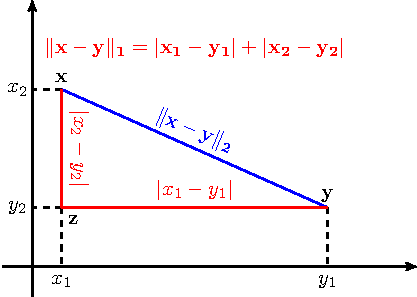
\includegraphics[width = .5\textwidth]{norm12.pdf}
			\caption{Minh họa norm 1 và norm 2}
			\label{fig:norm12}
		\end{figure}
		Norm 2 (màu xanh) chính là đường thằng "chim bay" nối giữa hai vector $\mathbf{x} $ và $\mathbf{y}$. Khoảng cách norm 1 giữa hai điểm này (màu đỏ) có thể diễn giải như là đường đi từ $\mathbf{x} $ tới $\mathbf{y}$ trong một thành phố mà đường phố tạo thành hình bàn cờ. Chúng ta chỉ có cách đi dọc theo cạnh của bàn cờ mà không được đi thẳng. 
 	
 	\item Khi $p \rightarrow \infty $, ta có norm $p$ chính là trị tuyệt đối của phần tử lớn nhất của vector đó:
		\begin{equation} 
		\|\mathbf{x}\|_{\infty} = \max_{i = 1, 2, \dots, n} \|x_i\|
		\end{equation} 
 
\end{enumerate} 
 
\subsection{Chuẩn của ma trận}
Với một ma trận $\mathbf{A} \in \mathbb{R}^{m\times n}$, chuẩn thường được dùng nhất là chuẩn Frobenius, ký hiệu là $\|\mathbf{A}\|_F$ là căn bậc hai của tổng bình phương tất cả các phần tử của ma trận đó.  
\begin{equation*} 
\|\mathbf{A}\|_F = \sqrt{\sum_{i = 1}^m \sum_{j = 1}^n a_{ij}^2} 
\end{equation*} 
 
 
 
 
\section{Đạo hàm của hàm nhiều biến }
Trong mục này, chúng ta sẽ giả sử rằng các đạo hàm tồn tại. Chúng ta sẽ xét hai trường hợp: i) Hàm số nhận giá trị là ma trận (vector) và cho giá trị là một số thực vô hướng; và ii) Hàm số nhận giá trị là một số vô hướng hoặc vector và cho giá trị là một vector.  
 
 
\subsection{Hàm cho giá trị là một số vô hướng}
 
Đạo hàm (gradient) của một hàm số $f(\mathbf{x}): \mathbb{R}^n \rightarrow \mathbb{R}$ \textbf{theo vector} $\mathbf{x}$ được định nghĩa như sau:  
 
\begin{equation} 
	\label{eqn:grvector1}
	\nabla_{\mathbf{x}} f(\mathbf{x}) \triangleq  
	\left[ 
	\begin{matrix} 
	\frac{\partial f(\mathbf{x})}{\partial x_1} \\\ 
	\frac{\partial f(\mathbf{x})}{\partial x_2} \\\ 
	\vdots \\\ 
	\frac{\partial f(\mathbf{x})}{\partial x_n} 
	\end{matrix} 
	\right] \in \mathbb{R}^n 
\end{equation} 
trong đó $\frac{\partial f(\mathbf{x})}{\partial x_i}$ là đạo hàm của hàm số theo thành phần thứ $i$ của vector $\mathbf{x}$. Đạo hàm này được lấy khi giả sử tất cả các biến còn lại là hằng số. 
 
Nếu không có thêm biến nào trong hàm số, $\nabla_{\mathbf{x}}f(\mathbf{x})$ thường được viết gọn là $\nabla f(\mathbf{x})$. 
 
Điều quan trọng cần nhớ: \textbf{đạo hàm của hàm số này là một vector có cùng chiều với vector đang lấy đạo hàm}. Tức nếu vector viết ở dạng cột thì đạo hàm cũng phải viết ở dạng cột.  
 
Đạo hàm bậc hai (second-order gradient) của hàm số trên còn được gọi là \textit{Hessian} và được định nghĩa như sau:  
 
\begin{equation} 
\label{eqn:hessian1}
\nabla^2 f(\mathbf{x}) \triangleq 
\left[ 
\begin{matrix} 
    \frac{\partial^2 f(\mathbf{x})}{\partial x_1^2} & \frac{\partial^2 f(\mathbf{x})}{\partial x_1x_2} & \dots & \frac{\partial^2 f(\mathbf{x})}{\partial x_1x_n} \\\  
    \frac{\partial^2 f(\mathbf{x})}{\partial x_2x_1} & \frac{\partial^2 f(\mathbf{x})}{\partial x_2^2} & \dots & \frac{\partial^2 f(\mathbf{x})}{\partial x_2x_n} \\\  
    \vdots & \vdots & \ddots & \vdots \\\ 
    \frac{\partial^2 f(\mathbf{x})}{\partial x_nx_1} & \frac{\partial^2 f(\mathbf{x})}{\partial x_nx_2} & \dots & \frac{\partial^2 f(\mathbf{x})}{\partial x_n^2} \\\  
\end{matrix} 
\right] \in \mathbb{S}^{n}
\end{equation}  
với $\mathbb{S}^{n} \in \mathbb{R}^{n \times n}$ là tập các ma trận vuông đối xứng có số cột là $n$. 

Đạo hàm của một hàm số $f(\mathbf{X}): \mathbb{R}^{n \times m} \rightarrow \mathbb{R}$ \textbf{theo ma trận} $\mathbf{X}$ được định nghĩa là:  
\begin{equation}
\label{eqn:grmatrix1} 
\nabla f(\mathbf{X}) = 
\left[ 
\begin{matrix} 
    \frac{\partial f(\mathbf{X})}{\partial x_{11}} & \frac{\partial f(\mathbf{X})}{\partial x_{12}} & \dots & \frac{\partial f(\mathbf{X})}{\partial x_{1m}} \\\ 
    \frac{\partial f(\mathbf{X})}{\partial x_{21}} & \frac{\partial f(\mathbf{X})}{\partial x_{22}} & \dots & \frac{\partial f(\mathbf{X})}{\partial x_{2m}} \\\ 
    \vdots & \vdots & \ddots & \vdots \\\ 
    \frac{\partial f(\mathbf{X})}{\partial x_{n1}} & \frac{\partial f(\mathbf{X})}{\partial x_{n2}} & \dots & \frac{\partial f(\mathbf{X})}{\partial x_{nm}}  
\end{matrix} 
\right] \in \mathbb{R}^{n \times m}
\end{equation} 
 
Một lần nữa, đạo hàm của một hàm số theo ma trận là một ma trận có chiều giống với ma trận đó. 
 
Hiểu một cách đơn giản, đạo hàm của một hàm số (có đầu ra là 1 số vô hướng) theo một ma trận được tính như sau. Trước tiên, tính đạo hàm của hàm số đó theo từng thành phần của ma trận \textit{khi toàn bộ các thành phần khác được giả sử là hằng số}. Tiếp theo, ta \textit{ghép} các đạo hàm thành phần tính được thành một ma trận đúng theo thứ tự như trong ma trận đó. Chú ý rằng vector là một trường hợp của ma trận.  
 
\textbf{Ví dụ:} Xét hàm số: $f: \mathbb{R}^2 \rightarrow \mathbb{R}$, $f(\mathbf{x}) = x_1 ^2 + 2x_1x_2 + \sin(x_1) + 2$.  
 
Đạo hàm bậc nhất theo $\mathbf{x}$ của hàm số đó là:  
\begin{equation*} 
\nabla f(\mathbf{x}) = 
\left[ 
\begin{matrix} 
    \frac{\partial f(\mathbf{x})}{\partial x_1} \\\ 
    \frac{\partial f(\mathbf{x})}{\partial x_2} 
\end{matrix} 
\right] = \left[ 
\begin{matrix} 
    2x_1 + 2x_2 + \cos(x_1) \\\ 
    2x_1 
\end{matrix} 
\right] 
\end{equation*} 
 
Đạo hàm bậc hai theo $\mathbf{x}$, hay \textit{Hessian} là:  
\begin{equation*} 
\nabla^2 f(\mathbf{x}) =  
\left[ 
\begin{matrix} 
    \frac{\partial^2 f(\mathbf{x})}{\partial x_1^2} & \frac{\partial f^2(\mathbf{x})}{\partial x_1x_2} \\\ 
    \frac{\partial^2 f(\mathbf{x})}{\partial x_2x_1} & \frac{\partial f^2(\mathbf{x})}{\partial x_2^2} 
\end{matrix} 
\right] = 
\left[ 
\begin{matrix} 
    2 - \sin(x_1) & 2 \\\ 
    2 & 0  
\end{matrix} 
\right] 
\end{equation*} 
Chú ý rằng \textit{Hessian} luôn là một ma trận đối xứng.  
 
 
 
\subsection{Hàm cho giá trị là một vector }
 
Những hàm số cho giá trị là một vector được gọi là \textit{vector-valued function} trong tiếng Anh.  
 
Giả sử một hàm số với \textbf{đầu vào là một số thực} $v(x): \mathbb{R} \rightarrow \mathbb{R}^n $: 
\begin{equation} 
\label{eqn:vectorvalued}
v(x) =  
\left[ 
\begin{matrix} 
    v_1(x) \\\ 
    v_2(x) \\\ 
    \vdots \\\ 
    v_n(x) 
\end{matrix} 
\right] 
\end{equation} 
Đạo hàm của nó là một \textbf{vector hàng} như sau:  

\begin{equation} 
\label{eqn:grvectorvalued}
\nabla v(x) \triangleq  
\left[ 
\begin{matrix} 
    \frac{\partial v_1(x)}{\partial x} & \frac{\partial v_2(x)}{\partial x} & \dots & \frac{\partial v_n(x)}{\partial x} 
\end{matrix} 
\right]
\end{equation} 
Đạo hàm bậc hai của hàm số này có dạng: 
 
\begin{equation} 
	\label{eqn:hessianvectorvalued}
	\nabla^2 v(x) \triangleq  
	\left[ 
	\begin{matrix} 
	    \frac{\partial^2 v_1(x)}{\partial x^2} & \frac{\partial^2 v_2(x)}{\partial x^2} & \dots & \frac{\partial^2 v_n(x)}{\partial x^2} 
	\end{matrix} 
	\right] 
\end{equation} 
 
\textbf{Ví dụ:} Cho vector $\mathbf{a} \in \mathbb{R}^n$ và \textit{vector-valued function} $v(x) = x\mathbf{a}$, thế thì: 
\begin{equation} 
\nabla v(x) = \mathbf{a}^T, ~~~ \nabla^2 v(x) = \mathbf{0} \in \mathbb{R}^{n\times n} 
\end{equation} 
với $\mathbf{0}$ là ma trận với các thành phần đều là 0.  

Xét một \textit{vector-valued function} với \textbf{đầu vào là một vector} $h(\mathbf{x}):\mathbb{R}^k \rightarrow \mathbb{R}^n$, đạo hàm bậc nhất của nó là: 
\begin{eqnarray} 
\label{eqn:gdvectorvector}
\nabla h(\mathbf{x}) &\triangleq & 
\left[ 
\begin{matrix} 
    \frac{\partial h_1(\mathbf{x})}{\partial x_1} & \frac{\partial h_2(\mathbf{x})}{\partial x_1} & \dots & \frac{\partial h_n(\mathbf{x})}{\partial x_1} \\\  
    \frac{\partial h_1(\mathbf{x})}{\partial x_2} & \frac{\partial h_2(\mathbf{x})}{\partial x_2} & \dots & \frac{\partial h_n(\mathbf{x})}{\partial x_2} \\\  
    \vdots & \vdots & \ddots & \vdots \\\ 
    \frac{\partial h_1(\mathbf{x})}{\partial x_k} & \frac{\partial h_2(\mathbf{x})}{\partial x_k} & \dots & \frac{\partial h_n(\mathbf{x})}{\partial x_k} 
\end{matrix} 
\right]\\
\label{eqn:gdvectorvector_short}
& = &  
\left[ 
\begin{matrix} 
    \nabla h_1(\mathbf{x}) & \nabla h_2(\mathbf{x}) & \dots & \nabla h_n(\mathbf{x}) 
\end{matrix} 
\right] \in \mathbf{R}^{k\times n} 
\end{eqnarray} 
 
 
\textbf{Một quy tắc dễ nhớ ở đây là nếu một hàm số} $g: \mathbb{R}^m \rightarrow \mathbb{R}^n$ \textbf{thì đạo hàm của nó là một ma trận thuộc} $\mathbb{R}^{m \times n}$. 
 
Đạo hàm bậc hai của hàm số trên là một \textit{ma trận ba chiều}, tôi xin không đề cập ở đây.  
 

<hr> 
Với các hàm số \textit{matrix-valued} nhận giá trị đầu vào là ma trận, tôi cũng xin không đề cập ở đây. Tuy nhiên, ở phần dưới, khi tính toán đạo hàm cho các hàm cho giá trị là số thực, chúng ta vẫn có thể sẽ sử dụng khái niệm này. 
 
Trước khi đến phần tính đạo hàm của các hàm số thường gặp, chúng ta cần biết hai tính chất quan trọng khá giống với đạo hàm của hàm một biến được học trong chương trình cấp ba.  
 
 
\subsection{Hai tính chất quan trọng }
 
 
\subsubsection{Product rules}
Để cho tổng quát, ta giả sử biến đầu vào là một ma trận (vector và số thực là các trường hợp đặt biệt của ma trận). Giả sử rằng các hàm số có chiều phù hợp để các phép nhân thực hiện được. Ta có:  
 
\begin{equation} 
\label{eqn:productrules}
\nabla\left( f(\mathbf{X})^Tg(\mathbf{X}) \right) = \left(\nabla f(\mathbf{X})\right) g(\mathbf{X}) + \left(\nabla g(\mathbf{X})\right) f(\mathbf{X})  
\end{equation} 
 
Biểu thức này giống như biểu thức chúng ta đã quá quen thuộc: 
\begin{equation*} 
\left(f(x)g(x)\right)' = f'(x)g(x) + g'(x)f(x) 
\end{equation*} 
Chú ý rằng với vector và ma trận, chúng ta không được sử dụng tính chất giao hoán.  
 
 
\subsubsection{Chain rules }
Khi có các hàm hợp thì: 
\begin{equation} 
\label{eqn:chainrules}
\nabla_{\mathbf{X}} g(f(\mathbf{X})) = \nabla_{\mathbf{X}} f^T \nabla_{f}g ~~~ (15) 
\end{equation} 
 
Quy tắc này cũng giống với quy tắc trong hàm một biến:  
\begin{equation*} 
(g(f(x))' = f'(x)g'(f) 
\end{equation*} 
Nhắc lại rằng khi tính toán với ma trận, chúng ta cần chú ý tới chiều của các ma trận, và nhân ma trận không có tính chất giao hoán.  
 
\subsection{Đạo hàm của các hàm số thường gặp }
 
\subsubsection{$f(\mathbf{x}) = \mathbf{a}^T\mathbf{x}$}
 
Giả sử $\mathbf{a}, \mathbf{x} \in \mathbb{R}^n$, ta viết lại: 
\begin{equation*} 
f(\mathbf{x}) = \mathbf{a}^T\mathbf{x} = a_1 x_1 + a_2 x_2 + \dots + a_nx_n 
\end{equation*} 
Có thể nhận thấy rằng: 
\begin{equation*} 
\frac{\partial f(\mathbf{x})}{\partial x_i} = a_i, ~ \forall i = 1, 2\dots, n 
\end{equation*} 
Vậy nên: 
\begin{equation*} 
\nabla f(\mathbf{x}) =  
\left[ 
\begin{matrix} 
    a_1 \\\ 
    a_2 \\\ 
    \vdots \\\ 
    a_n 
\end{matrix} 
\right] = \mathbf{a}
\end{equation*} 
 
Thêm nữa, vì $\mathbf{a}^T\mathbf{x} = \mathbf{x}^T\mathbf{a}$ nên: 
\begin{equation*} 
\nabla (\mathbf{x}^T\mathbf{a}) = \mathbf{a} 
\end{equation*} 
 
 
\subsubsection{$f(\mathbf{x}) = \mathbf{Ax}$}
Đây là một \textit{vector-valued function} $f: \mathbb{R}^n \rightarrow \mathbb{R}^{m} $ với $\mathbf{x} \in \mathbb{R}^n, \mathbf{A} \in \mathbb{R}^{m\times n}$. Giả sử rằng $\mathbf{a}_i$ là \textbf{hàng} thứ $i$ của ma trận $\mathbf{A}$. Ta có:  
\begin{equation*} 
\mathbf{Ax}  =  
\left[ 
\begin{matrix} 
    \mathbf{a}_1\mathbf{x} \\\ 
    \mathbf{a}_2\mathbf{x} \\\ 
    \vdots\\\ 
    \mathbf{a}_m\mathbf{x}  
\end{matrix} 
\right] 
\end{equation*} 
Theo định nghĩa $(13.2)$, và công thức $(17)$, ta có thể suy ra: 
\begin{equation} 
\label{eqn:gdAx}
\nabla_{\mathbf{x}} (\mathbf{Ax}) =  
\left[ 
\begin{matrix} 
    \mathbf{a}_1^T & \mathbf{a}_2^T & \dots & \mathbf{a}_m^T 
\end{matrix} 
\right] = \mathbf{A}^T 
\end{equation} 
 
Từ đây ta có thể suy ra đạo hàm của hàm số $f(\mathbf{x}) = \mathbf{x} = \mathbf{Ix}$, với $\mathbf{I}$ là ma trận đơn vị với chiều phù hợp, là: 
\begin{equation*} 
\nabla \mathbf{x} = \mathbf{I} 
\end{equation*} 
 
\subsubsection{$f(\mathbf{x}) = \mathbf{x}^T\mathbf{A} \mathbf{x}$}
với $\mathbf{x} \in \mathbb{R}^n, \mathbf{A} \in \mathbb{R}^{n\times n}$. Áp dụng Product rules $(14)$ ta có: 
\begin{eqnarray} 
	\nonumber
	\nabla f(\mathbf{x}) &=& \nabla \left(\left(\mathbf{x}^T\right) \left(\mathbf{Ax}\right)\right) \\\ 
				\nonumber
                     &=& \left(\nabla (\mathbf{x})\right) \mathbf{Ax} + \left(\nabla (\mathbf{Ax})\right)\mathbf{x} \\\  
					\nonumber
                     & = & \mathbf{IAx} + \mathbf{A}^T\mathbf{x} \\\ 
                     \label{eqn:gdxTAx}
                     & = & (\mathbf{A} + \mathbf{A}^T)\mathbf{x} 
\end{eqnarray} 
 
 
Từ \eqref{eqn:gdxTAx} và \eqref{eqn:gdAx}, ta có thể suy ra:  
\begin{math} 
\nabla^2 \mathbf{x}^T\mathbf{Ax} = \mathbf{A}^T + \mathbf{A} 
\end{math} 
 
Nếu $\mathbf{A}$ là một ma trận đối xứng, ta sẽ có: 
\begin{equation} 
\nabla \mathbf{x}^T\mathbf{A}\mathbf{x} = 2\mathbf{Ax}, ~~~
\nabla^2 \mathbf{x}^T\mathbf{Ax} = 2\mathbf{A} 
\end{equation} 
 
Nếu $\mathbf{A}$ là ma trận đơn vị, tức $f(\mathbf{x}) = \mathbf{x}^T\mathbf{Ix} = \mathbf{x}^T\mathbf{x} = \|\mathbf{x}\|_2^2$, ta có: 
\begin{equation} 
\nabla \|\mathbf{x}\|_2^2 = 2\mathbf{x},~~~
\nabla^2 \|\mathbf{x}\|_2^2 = 2\mathbf{I} 
\end{equation} 
 
 
\subsubsection{$f(\mathbf{x}) = \|\mathbf{Ax} - \mathbf{b}\|_2^2 $}
Có hai cách tính đạo hàm của hàm số này: 
 
\textbf{Cách 1:} 
Trước hết, biến đổi: 
\begin{eqnarray} 
	\nonumber
	f(\mathbf{x}) &=& \|\mathbf{Ax} - \mathbf{b}\|_2^2 = (\mathbf{Ax} - \mathbf{b})^T(\mathbf{Ax} - \mathbf{b}) = (\mathbf{x}^T\mathbf{A}^T - \mathbf{b}^T) (\mathbf{Ax} - \mathbf{b}) \\\ \nonumber
	&=& \mathbf{x}^T\mathbf{A}^T\mathbf{Ax} - 2 \mathbf{b}^T\mathbf{Ax} + \mathbf{b}^T\mathbf{b} 
\end{eqnarray} 
Lấy đạo hàm cho từng số hạng rồi cộng lại ta có:  
\begin{equation*} 
\nabla \|\mathbf{Ax} - \mathbf{b}\|_2^2 = 2\mathbf{A}^T\mathbf{A}\mathbf{x} - 2\mathbf{A}^T\mathbf{b} = 2\mathbf{A}^T(\mathbf{Ax} - \mathbf{b}) 
\end{equation*} 
 
\textbf{Cách 2:} Dùng Chain rule. 
Sử dụng $\nabla (\mathbf{Ax} - \mathbf{b}) = \mathbf{A}^T$ và $\nabla \|\mathbf{x}\|_2^2 = 2\mathbf{x}$ và công thức chain rules \eqref{eqn:chainrules}, ta sẽ thu được kết quả tương tự.  
 
 
\subsubsection{$f(\mathbf{x}) = \mathbf{a}^T\mathbf{x}\mathbf{x}^T\mathbf{b}$}
Bằng cách viết lại $f(\mathbf{x}) = (\mathbf{a}^T\mathbf{x})(\mathbf{x}^T\mathbf{b})$, ta có thể dùng Product rules $(14)$ và ra kết quả:  
\begin{equation*} 
	\nabla (\mathbf{a}^T\mathbf{x}\mathbf{x}^T\mathbf{b}) = \mathbf{a} \mathbf{x}^T\mathbf{b} +  \mathbf{b}\mathbf{a}^T\mathbf{x} = \mathbf{ab}^T\mathbf{x} + \mathbf{b}\mathbf{a}^T\mathbf{x}= (\mathbf{ab}^T + \mathbf{ba}^T)\mathbf{x} 
\end{equation*} 
trong đây tôi đã sử dụng tính chất $\mathbf{y}^T\mathbf{z} = \mathbf{z}^T\mathbf{y}$ và tích của một số thực với một vector cũng bằng tích của vector và số thực đó.  
 
 
\subsection{Bảng các đạo hàm thường gặp}
 
\subsubsection{Cho vector }
 
\begin{table}[h!]
\centering
\caption{Đạo hàm theo vector}
\label{my-label}
\begin{tabular}{|c|c|}
\hline
$f(\mathbf{x}) $                                                                          & $ \nabla f(\mathbf{x}) $                                         \\ \hline
$\mathbf{a}^T \mathbf{x} $                                                                & $\mathbf{a}$                                                     \\ \hline
$\mathbf{x}^T\mathbf{Ax}$                                                                 & $\mathbf{A} + \mathbf{A}^T) \mathbf{x}$                          \\ \hline
$\mathbf{x}^T \mathbf{x} = \|\mathbf{x}\|_2^2 $ & $2\mathbf{x}$                                                   \\ \hline
$ \|\mathbf{Ax-b} \|_2^2 $                                                                & $ 2\mathbf{A}^T (\mathbf{Ax - b})$                               \\ \hline
$\mathbf{a}^T\mathbf{x}^T\mathbf{xb} $                                                    & $2\mathbf{a}^T\mathbf{bx} $                                      \\ \hline
$\mathbf{a}^T\mathbf{x}\mathbf{x}^T\mathbf{b} $                                           & $ (\mathbf{a}\mathbf{b}^T + \mathbf{b}\mathbf{a}^T) \mathbf{x} $ \\ \hline
\end{tabular}
\end{table}


 
\subsubsection{Cho ma trận}
 

 \begin{table}[h!]
\centering
\caption{Đạo hàm theo ma trận}
\label{my-label}
\begin{tabular}{|c|c|}
\hline
$f(\mathbf{X}) $                                   & $ \nabla f(\mathbf{X}) $                      \\ \hline
$ \|\mathbf{X}\|_F^2$ & $2\mathbf{X}$ \\\hline
$ \mathbf{AX}$ & $\mathbf{A}^T$ \\\hline
$ \|\mathbf{AX - B}\|_F^2$ & $2\mathbf{A}^T(\mathbf{AX - B})$ \\\hline
$ \|\mathbf{XA - B}\|_F^2$ & $2(\mathbf{XA-B})\mathbf{A}^T$ \\\hline
$ \mathbf{a}^T \mathbf{X}^T \mathbf{Xb}$           & $ \mathbf{X}(\mathbf{ab}^T + \mathbf{ba}^T)$ \\ \hline
$ \mathbf{a}^T \mathbf{X} \mathbf{X}^T \mathbf{b}$ & $ (\mathbf{ab}^T + \mathbf{ba}^T)\mathbf{X},$ \\ \hline
$ \mathbf{a}^T \mathbf{Y} \mathbf{X}^T \mathbf{b}$ & $ \mathbf{b}\mathbf{a}^T \mathbf{Y}$         \\ \hline
$ \mathbf{a}^T \mathbf{Y}^T \mathbf{X} \mathbf{b}$ & $ \mathbf{Y}\mathbf{a}\mathbf{b}^T$          \\ \hline
$ \mathbf{a}^T \mathbf{X} \mathbf{Y}^T \mathbf{b}$ & $ \mathbf{a}\mathbf{b}^T\mathbf{Y}$          \\ \hline
$ \mathbf{a}^T \mathbf{X}^T \mathbf{Y} \mathbf{b}$ & $ \mathbf{Y}\mathbf{b}\mathbf{a}^T$          \\ \hline
\end{tabular}
\end{table}


\subsection{Tài liệu tham khảo }
[1] \href{https://ccrma.stanford.edu/~dattorro/matrixcalc.pdf}{Matrix calculus} 
 
 
 

\end{document}

\backmatter%%%%%%%%%%%%%%%%%%%%%%%%%%%%%%%%%%%%%%%%%%%%%%%%%%%%%%%
% 
\chapter*{Solutions}
\addcontentsline{toc}{chapter}{Solutions}
\markboth{Solutions}{Solutions}

\section*{Problems of Chapter~\ref{intro}}

\begin{sol}{prob1}
The solution is revealed here.
\end{sol}


\begin{sol}{prob2}
\textbf{Problem Heading}\\
(a) The solution of first part is revealed here.\\
(b) The solution of second part is revealed here.
\end{sol}


% %%%%%%%%%%%%%%%%%%%%%%%% referenc.tex %%%%%%%%%%%%%%%%%%%%%%%%%%%%%%
% sample references
% "computer science"
%
% Use this file as a template for your own input.
%
%%%%%%%%%%%%%%%%%%%%%%%% Springer-Verlag %%%%%%%%%%%%%%%%%%%%%%%%%%

%
% BibTeX users please use
% \bibliographystyle{}
% \bibliography{}
%
% Non-BibTeX users please use
\begin{thebibliography}{99.}
%
% and use \bibitem to create references.
%
% Use the following syntax and markup for your references
%
% Monographs
\bibitem{monograph} Kajan E (2002)
Information technology encyclopedia and acronyms. Springer, Berlin
Heidelberg New York

% Contributed Works
\bibitem{contribution} Broy M (2002) Software engineering -- From
auxiliary to key technologies. In: Broy M, Denert E (eds)
Software Pioneers. Springer, Berlin Heidelberg New York

% Journal
\bibitem{journal} Che M, Grellmann W, Seidler S (1997)
Appl Polym Sci 64:1079--1090

% Theses
\bibitem{thesis} Ross DW (1977) Lysosomes and storage diseases. MA
Thesis, Columbia University, New York

\end{thebibliography}

\printindex

%%%%%%%%%%%%%%%%%%%%%%%%%%%%%%%%%%%%%%%%%%%%%%%%%%%%%%%%%%%%%%%%%%%%%%

\end{document}





